% Options for packages loaded elsewhere
\PassOptionsToPackage{unicode}{hyperref}
\PassOptionsToPackage{hyphens}{url}
\PassOptionsToPackage{dvipsnames,svgnames,x11names}{xcolor}
%
\documentclass[
  letterpaper,
]{krantz}

\usepackage{amsmath,amssymb}
\usepackage{iftex}
\ifPDFTeX
  \usepackage[T1]{fontenc}
  \usepackage[utf8]{inputenc}
  \usepackage{textcomp} % provide euro and other symbols
\else % if luatex or xetex
  \usepackage{unicode-math}
  \defaultfontfeatures{Scale=MatchLowercase}
  \defaultfontfeatures[\rmfamily]{Ligatures=TeX,Scale=1}
\fi
\usepackage{lmodern}
\ifPDFTeX\else  
    % xetex/luatex font selection
\fi
% Use upquote if available, for straight quotes in verbatim environments
\IfFileExists{upquote.sty}{\usepackage{upquote}}{}
\IfFileExists{microtype.sty}{% use microtype if available
  \usepackage[]{microtype}
  \UseMicrotypeSet[protrusion]{basicmath} % disable protrusion for tt fonts
}{}
\makeatletter
\@ifundefined{KOMAClassName}{% if non-KOMA class
  \IfFileExists{parskip.sty}{%
    \usepackage{parskip}
  }{% else
    \setlength{\parindent}{0pt}
    \setlength{\parskip}{6pt plus 2pt minus 1pt}}
}{% if KOMA class
  \KOMAoptions{parskip=half}}
\makeatother
\usepackage{xcolor}
\setlength{\emergencystretch}{3em} % prevent overfull lines
\setcounter{secnumdepth}{5}
% Make \paragraph and \subparagraph free-standing
\ifx\paragraph\undefined\else
  \let\oldparagraph\paragraph
  \renewcommand{\paragraph}[1]{\oldparagraph{#1}\mbox{}}
\fi
\ifx\subparagraph\undefined\else
  \let\oldsubparagraph\subparagraph
  \renewcommand{\subparagraph}[1]{\oldsubparagraph{#1}\mbox{}}
\fi

\usepackage{color}
\usepackage{fancyvrb}
\newcommand{\VerbBar}{|}
\newcommand{\VERB}{\Verb[commandchars=\\\{\}]}
\DefineVerbatimEnvironment{Highlighting}{Verbatim}{commandchars=\\\{\}}
% Add ',fontsize=\small' for more characters per line
\usepackage{framed}
\definecolor{shadecolor}{RGB}{241,243,245}
\newenvironment{Shaded}{\begin{snugshade}}{\end{snugshade}}
\newcommand{\AlertTok}[1]{\textcolor[rgb]{0.68,0.00,0.00}{#1}}
\newcommand{\AnnotationTok}[1]{\textcolor[rgb]{0.37,0.37,0.37}{#1}}
\newcommand{\AttributeTok}[1]{\textcolor[rgb]{0.40,0.45,0.13}{#1}}
\newcommand{\BaseNTok}[1]{\textcolor[rgb]{0.68,0.00,0.00}{#1}}
\newcommand{\BuiltInTok}[1]{\textcolor[rgb]{0.00,0.23,0.31}{#1}}
\newcommand{\CharTok}[1]{\textcolor[rgb]{0.13,0.47,0.30}{#1}}
\newcommand{\CommentTok}[1]{\textcolor[rgb]{0.37,0.37,0.37}{#1}}
\newcommand{\CommentVarTok}[1]{\textcolor[rgb]{0.37,0.37,0.37}{\textit{#1}}}
\newcommand{\ConstantTok}[1]{\textcolor[rgb]{0.56,0.35,0.01}{#1}}
\newcommand{\ControlFlowTok}[1]{\textcolor[rgb]{0.00,0.23,0.31}{#1}}
\newcommand{\DataTypeTok}[1]{\textcolor[rgb]{0.68,0.00,0.00}{#1}}
\newcommand{\DecValTok}[1]{\textcolor[rgb]{0.68,0.00,0.00}{#1}}
\newcommand{\DocumentationTok}[1]{\textcolor[rgb]{0.37,0.37,0.37}{\textit{#1}}}
\newcommand{\ErrorTok}[1]{\textcolor[rgb]{0.68,0.00,0.00}{#1}}
\newcommand{\ExtensionTok}[1]{\textcolor[rgb]{0.00,0.23,0.31}{#1}}
\newcommand{\FloatTok}[1]{\textcolor[rgb]{0.68,0.00,0.00}{#1}}
\newcommand{\FunctionTok}[1]{\textcolor[rgb]{0.28,0.35,0.67}{#1}}
\newcommand{\ImportTok}[1]{\textcolor[rgb]{0.00,0.46,0.62}{#1}}
\newcommand{\InformationTok}[1]{\textcolor[rgb]{0.37,0.37,0.37}{#1}}
\newcommand{\KeywordTok}[1]{\textcolor[rgb]{0.00,0.23,0.31}{#1}}
\newcommand{\NormalTok}[1]{\textcolor[rgb]{0.00,0.23,0.31}{#1}}
\newcommand{\OperatorTok}[1]{\textcolor[rgb]{0.37,0.37,0.37}{#1}}
\newcommand{\OtherTok}[1]{\textcolor[rgb]{0.00,0.23,0.31}{#1}}
\newcommand{\PreprocessorTok}[1]{\textcolor[rgb]{0.68,0.00,0.00}{#1}}
\newcommand{\RegionMarkerTok}[1]{\textcolor[rgb]{0.00,0.23,0.31}{#1}}
\newcommand{\SpecialCharTok}[1]{\textcolor[rgb]{0.37,0.37,0.37}{#1}}
\newcommand{\SpecialStringTok}[1]{\textcolor[rgb]{0.13,0.47,0.30}{#1}}
\newcommand{\StringTok}[1]{\textcolor[rgb]{0.13,0.47,0.30}{#1}}
\newcommand{\VariableTok}[1]{\textcolor[rgb]{0.07,0.07,0.07}{#1}}
\newcommand{\VerbatimStringTok}[1]{\textcolor[rgb]{0.13,0.47,0.30}{#1}}
\newcommand{\WarningTok}[1]{\textcolor[rgb]{0.37,0.37,0.37}{\textit{#1}}}

\providecommand{\tightlist}{%
  \setlength{\itemsep}{0pt}\setlength{\parskip}{0pt}}\usepackage{longtable,booktabs,array}
\usepackage{calc} % for calculating minipage widths
% Correct order of tables after \paragraph or \subparagraph
\usepackage{etoolbox}
\makeatletter
\patchcmd\longtable{\par}{\if@noskipsec\mbox{}\fi\par}{}{}
\makeatother
% Allow footnotes in longtable head/foot
\IfFileExists{footnotehyper.sty}{\usepackage{footnotehyper}}{\usepackage{footnote}}
\makesavenoteenv{longtable}
\usepackage{graphicx}
\makeatletter
\def\maxwidth{\ifdim\Gin@nat@width>\linewidth\linewidth\else\Gin@nat@width\fi}
\def\maxheight{\ifdim\Gin@nat@height>\textheight\textheight\else\Gin@nat@height\fi}
\makeatother
% Scale images if necessary, so that they will not overflow the page
% margins by default, and it is still possible to overwrite the defaults
% using explicit options in \includegraphics[width, height, ...]{}
\setkeys{Gin}{width=\maxwidth,height=\maxheight,keepaspectratio}
% Set default figure placement to htbp
\makeatletter
\def\fps@figure{htbp}
\makeatother

\usepackage{booktabs}
\usepackage{longtable}
\usepackage[bf,singlelinecheck=off]{caption}
\usepackage[scale=.8]{sourcecodepro}
\usepackage{hyperref}

\usepackage{framed,color}
\definecolor{shadecolor}{RGB}{248,248,248}

\renewcommand{\textfraction}{0.05}
\renewcommand{\topfraction}{0.8}
\renewcommand{\bottomfraction}{0.8}
\renewcommand{\floatpagefraction}{0.75}

\renewenvironment{quote}{\begin{VF}}{\end{VF}}
\let\oldhref\href
\renewcommand{\href}[2]{#2\footnote{\url{#1}}}

\makeatletter
\newenvironment{kframe}{%
\medskip{}
\setlength{\fboxsep}{.8em}
 \def\at@end@of@kframe{}%
 \ifinner\ifhmode%
  \def\at@end@of@kframe{\end{minipage}}%
  \begin{minipage}{\columnwidth}%
 \fi\fi%
 \def\FrameCommand##1{\hskip\@totalleftmargin \hskip-\fboxsep
 \colorbox{shadecolor}{##1}\hskip-\fboxsep
     % There is no \\@totalrightmargin, so:
     \hskip-\linewidth \hskip-\@totalleftmargin \hskip\columnwidth}%
 \MakeFramed {\advance\hsize-\width
   \@totalleftmargin\z@ \linewidth\hsize
   \@setminipage}}%
 {\par\unskip\endMakeFramed%
 \at@end@of@kframe}
\makeatother

\renewenvironment{Shaded}{\begin{kframe}}{\end{kframe}}

\usepackage{makeidx}
\makeindex

\urlstyle{tt}

\usepackage{amsthm}
\makeatletter
\def\thm@space@setup{%
  \thm@preskip=8pt plus 2pt minus 4pt
  \thm@postskip=\thm@preskip
}
\makeatother

\frontmatter
\makeatletter
\makeatother
\makeatletter
\@ifpackageloaded{bookmark}{}{\usepackage{bookmark}}
\makeatother
\makeatletter
\@ifpackageloaded{caption}{}{\usepackage{caption}}
\AtBeginDocument{%
\ifdefined\contentsname
  \renewcommand*\contentsname{Table of contents}
\else
  \newcommand\contentsname{Table of contents}
\fi
\ifdefined\listfigurename
  \renewcommand*\listfigurename{List of Figures}
\else
  \newcommand\listfigurename{List of Figures}
\fi
\ifdefined\listtablename
  \renewcommand*\listtablename{List of Tables}
\else
  \newcommand\listtablename{List of Tables}
\fi
\ifdefined\figurename
  \renewcommand*\figurename{Figure}
\else
  \newcommand\figurename{Figure}
\fi
\ifdefined\tablename
  \renewcommand*\tablename{Table}
\else
  \newcommand\tablename{Table}
\fi
}
\@ifpackageloaded{float}{}{\usepackage{float}}
\floatstyle{ruled}
\@ifundefined{c@chapter}{\newfloat{codelisting}{h}{lop}}{\newfloat{codelisting}{h}{lop}[chapter]}
\floatname{codelisting}{Listing}
\newcommand*\listoflistings{\listof{codelisting}{List of Listings}}
\makeatother
\makeatletter
\@ifpackageloaded{caption}{}{\usepackage{caption}}
\@ifpackageloaded{subcaption}{}{\usepackage{subcaption}}
\makeatother
\makeatletter
\@ifpackageloaded{tcolorbox}{}{\usepackage[skins,breakable]{tcolorbox}}
\makeatother
\makeatletter
\@ifundefined{shadecolor}{\definecolor{shadecolor}{rgb}{.97, .97, .97}}
\makeatother
\makeatletter
\makeatother
\makeatletter
\makeatother
\ifLuaTeX
  \usepackage{selnolig}  % disable illegal ligatures
\fi
\IfFileExists{bookmark.sty}{\usepackage{bookmark}}{\usepackage{hyperref}}
\IfFileExists{xurl.sty}{\usepackage{xurl}}{} % add URL line breaks if available
\urlstyle{same} % disable monospaced font for URLs
\hypersetup{
  pdftitle={Proyek Sains Data},
  pdfauthor={Akhmad Raihan Aulia Fikri 20-095},
  colorlinks=true,
  linkcolor={blue},
  filecolor={Maroon},
  citecolor={Blue},
  urlcolor={Blue},
  pdfcreator={LaTeX via pandoc}}

\title{Proyek Sains Data}
\author{Akhmad Raihan Aulia Fikri 20-095}
\date{2024-08-11}

\begin{document}
\maketitle
% you may need to leave a few empty pages before the dedication page

%\cleardoublepage\newpage\thispagestyle{empty}\null
%\cleardoublepage\newpage\thispagestyle{empty}\null
%\cleardoublepage\newpage
\thispagestyle{empty}

\begin{center}
To blah, blah, and blah.
%\includegraphics{images/dedication.pdf}
\end{center}

\setlength{\abovedisplayskip}{-5pt}
\setlength{\abovedisplayshortskip}{-5pt}

\ifdefined\Shaded\renewenvironment{Shaded}{\begin{tcolorbox}[boxrule=0pt, enhanced, sharp corners, frame hidden, breakable, interior hidden, borderline west={3pt}{0pt}{shadecolor}]}{\end{tcolorbox}}\fi

\renewcommand*\contentsname{Table of contents}
{
\hypersetup{linkcolor=}
\setcounter{tocdepth}{2}
\tableofcontents
}
\bookmarksetup{startatroot}

\hypertarget{introduction}{%
\chapter*{Introduction}\label{introduction}}
\addcontentsline{toc}{chapter}{Introduction}

\markboth{Introduction}{Introduction}

PSD by Posit

Model Via Streamlit : Klasifikasi Hewan \mainmatter

\bookmarksetup{startatroot}

\hypertarget{zoo}{%
\chapter{Zoo}\label{zoo}}

\hypertarget{business-understanding}{%
\section{Business Understanding}\label{business-understanding}}

Tujuan utama dari proyek ini adalah mengembangkan model klasifikasi
untuk mengidentifikasi kategori hewan berdasarkan fitur fitur yang ada.
Hasil dari model ini dapat digunakan untuk beberapa hal seperti:

\begin{itemize}
\tightlist
\item
  Membantu ahli biologi atau peneliti dalam mengidentifikasi hewan
\item
  Menyediakan alat untuk mengidentifikasi hewan sesuai spesies dan
  klasifikasinya
\end{itemize}

\hypertarget{data-understanding}{%
\section{Data Understanding}\label{data-understanding}}

Dataset yang saya gunakan yaitu data Zoo dari website UCI Machine
Learning. Data ini merupakan sebuah dataset sederhana untuk
mengklasifikasikan hewan berdasarkan 17 atribut bertipe boolean dan 1
atribut numerik. Dataset yang digunakan memiliki 101 data.

\hypertarget{penjelasan-atribut}{%
\subsection{Penjelasan atribut}\label{penjelasan-atribut}}

Berikut ini adalah penjelasan atribut atribut yang digunakan

\begin{itemize}
\tightlist
\item
  Hair = Rambut \emph{(Boolean)}
\end{itemize}

\begin{verbatim}
0 = Tidak
1 = Ya
\end{verbatim}

\begin{itemize}
\tightlist
\item
  Feathers = Bulu \emph{(Boolean)}
\end{itemize}

\begin{verbatim}
0 = Tidak
1 = Ya
\end{verbatim}

\begin{itemize}
\tightlist
\item
  Eggs = Bertelur \emph{(Boolean)}
\end{itemize}

\begin{verbatim}
0 = Tidak
1 = Ya
\end{verbatim}

\begin{itemize}
\tightlist
\item
  Milk = Menyusui \emph{(Boolean)}
\end{itemize}

\begin{verbatim}
0 = Tidak
1 = Ya
\end{verbatim}

\begin{itemize}
\tightlist
\item
  Airbone = Mengudara \emph{(Boolean)}
\end{itemize}

\begin{verbatim}
0 = Tidak
1 = Ya
\end{verbatim}

\begin{itemize}
\tightlist
\item
  Aquatic = Akuatik \emph{(Boolean)}
\end{itemize}

\begin{verbatim}
0 = Tidak
1 = Ya
\end{verbatim}

\begin{itemize}
\tightlist
\item
  Predator = Predator \emph{(Boolean)}
\end{itemize}

\begin{verbatim}
0 = Tidak
1 = Ya
\end{verbatim}

\begin{itemize}
\tightlist
\item
  Toothed = Bergigi \emph{(Boolean)}
\end{itemize}

\begin{verbatim}
0 = Tidak
1 = Ya
\end{verbatim}

\begin{itemize}
\tightlist
\item
  Backbone = Tulang belakang \emph{(Boolean)}
\end{itemize}

\begin{verbatim}
0 = Tidak
1 = Ya
\end{verbatim}

\begin{itemize}
\tightlist
\item
  Breathes = Bernafas \emph{(Boolean)}
\end{itemize}

\begin{verbatim}
0 = Tidak
1 = Ya
\end{verbatim}

\begin{itemize}
\tightlist
\item
  Venomous = Beracun \emph{(Boolean)}
\end{itemize}

\begin{verbatim}
0 = Tidak
1 = Ya
\end{verbatim}

\begin{itemize}
\tightlist
\item
  Fins = Sirip \emph{(Boolean)}
\end{itemize}

\begin{verbatim}
0 = Tidak
1 = Ya
\end{verbatim}

\begin{itemize}
\tightlist
\item
  Legs = Kaki \emph{(Numerical)}
\end{itemize}

\begin{verbatim}
0 , 1 , 2 , 3, 4 , 5 , 6 , 7 , 8 dst
\end{verbatim}

\begin{itemize}
\tightlist
\item
  Tail = Berekor \emph{(Boolean)}
\end{itemize}

\begin{verbatim}
0 = Tidak
1 = Ya
\end{verbatim}

\begin{itemize}
\tightlist
\item
  Domestic = Jinak \emph{(Boolean)}
\end{itemize}

\begin{verbatim}
0 = Tidak
1 = Ya
\end{verbatim}

\begin{itemize}
\tightlist
\item
  Catsize = Ukuran kucing \emph{(Boolean)}
\end{itemize}

\begin{verbatim}
0 = Tidak
1 = Ya
\end{verbatim}

\hypertarget{data-preparation}{%
\section{Data Preparation}\label{data-preparation}}

\hypertarget{library-uci-machine-learning}{%
\subsection{Library uci machine
learning}\label{library-uci-machine-learning}}

\begin{Shaded}
\begin{Highlighting}[]
\OperatorTok{!}\NormalTok{pip install ucimlrepo}
\end{Highlighting}
\end{Shaded}

\begin{verbatim}
Requirement already satisfied: ucimlrepo in /usr/local/lib/python3.10/dist-packages (0.0.3)
\end{verbatim}

\begin{Shaded}
\begin{Highlighting}[]
\ImportTok{import}\NormalTok{ matplotlib.pyplot }\ImportTok{as}\NormalTok{ plt}
\ImportTok{import}\NormalTok{ pandas }\ImportTok{as}\NormalTok{ pd}
\ImportTok{import}\NormalTok{ seaborn }\ImportTok{as}\NormalTok{ sns}
\ImportTok{import}\NormalTok{ numpy }\ImportTok{as}\NormalTok{ np}
\end{Highlighting}
\end{Shaded}

\hypertarget{install-dataset-zoo-otomatis}{%
\subsection{Install dataset Zoo
otomatis}\label{install-dataset-zoo-otomatis}}

Penginstallan dataset zoo ini menggunakan X sebagai data fitur dan y
sebagai target. Data yang dipakai tidak memiliki missing values sehingga
bisa lanjut ke tahap preprocessing selanjutnya

\begin{Shaded}
\begin{Highlighting}[]
\ImportTok{from}\NormalTok{ ucimlrepo }\ImportTok{import}\NormalTok{ fetch\_ucirepo}

\CommentTok{\# fetch dataset}
\NormalTok{zoo }\OperatorTok{=}\NormalTok{ fetch\_ucirepo(}\BuiltInTok{id}\OperatorTok{=}\DecValTok{111}\NormalTok{)}

\CommentTok{\# data (as pandas dataframes)}
\NormalTok{X }\OperatorTok{=}\NormalTok{ zoo.data.features}
\NormalTok{y }\OperatorTok{=}\NormalTok{ zoo.data.targets}


\CommentTok{\# metadata}
\BuiltInTok{print}\NormalTok{(zoo.metadata)}

\CommentTok{\# variable information}
\BuiltInTok{print}\NormalTok{(zoo.variables)}
\end{Highlighting}
\end{Shaded}

\begin{verbatim}
{'uci_id': 111, 'name': 'Zoo', 'repository_url': 'https://archive.ics.uci.edu/dataset/111/zoo', 'data_url': 'https://archive.ics.uci.edu/static/public/111/data.csv', 'abstract': 'Artificial, 7 classes of animals', 'area': 'Biology', 'tasks': ['Classification'], 'characteristics': ['Multivariate'], 'num_instances': 101, 'num_features': 16, 'feature_types': ['Categorical', 'Integer'], 'demographics': [], 'target_col': ['type'], 'index_col': ['animal_name'], 'has_missing_values': 'no', 'missing_values_symbol': None, 'year_of_dataset_creation': 1990, 'last_updated': 'Fri Sep 15 2023', 'dataset_doi': '10.24432/C5R59V', 'creators': ['Richard Forsyth'], 'intro_paper': None, 'additional_info': {'summary': 'A simple database containing 17 Boolean-valued attributes.  The "type" attribute appears to be the class attribute.  Here is a breakdown of which animals are in which type: (I find it unusual that there are 2 instances of "frog" and one of "girl"!)', 'purpose': None, 'funded_by': None, 'instances_represent': None, 'recommended_data_splits': None, 'sensitive_data': None, 'preprocessing_description': None, 'variable_info': '   1. animal name:      Unique for each instance\r\n   2. hair:\t\tBoolean\r\n   3. feathers:\t\tBoolean\r\n   4. eggs:\t\tBoolean\r\n   5. milk:\t\tBoolean\r\n   6. airborne:\t\tBoolean\r\n   7. aquatic:\t\tBoolean\r\n   8. predator:\t\tBoolean\r\n   9. toothed:\t\tBoolean\r\n  10. backbone:\t\tBoolean\r\n  11. breathes:\t\tBoolean\r\n  12. venomous:\t\tBoolean\r\n  13. fins:\t\tBoolean\r\n  14. legs:\t\tNumeric (set of values: {0,2,4,5,6,8})\r\n  15. tail:\t\tBoolean\r\n  16. domestic:\t\tBoolean\r\n  17. catsize:\t\tBoolean\r\n  18. type:\t\tNumeric (integer values in range [1,7])', 'citation': None}}
           name     role         type demographic description units  \
0   animal_name       ID  Categorical        None        None  None   
1          hair  Feature       Binary        None        None  None   
2      feathers  Feature       Binary        None        None  None   
3          eggs  Feature       Binary        None        None  None   
4          milk  Feature       Binary        None        None  None   
5      airborne  Feature       Binary        None        None  None   
6       aquatic  Feature       Binary        None        None  None   
7      predator  Feature       Binary        None        None  None   
8       toothed  Feature       Binary        None        None  None   
9      backbone  Feature       Binary        None        None  None   
10     breathes  Feature       Binary        None        None  None   
11     venomous  Feature       Binary        None        None  None   
12         fins  Feature       Binary        None        None  None   
13         legs  Feature  Categorical        None        None  None   
14         tail  Feature       Binary        None        None  None   
15     domestic  Feature       Binary        None        None  None   
16      catsize  Feature       Binary        None        None  None   
17         type   Target  Categorical        None        None  None   

   missing_values  
0              no  
1              no  
2              no  
3              no  
4              no  
5              no  
6              no  
7              no  
8              no  
9              no  
10             no  
11             no  
12             no  
13             no  
14             no  
15             no  
16             no  
17             no  
\end{verbatim}

\begin{Shaded}
\begin{Highlighting}[]
\CommentTok{\# URL dataset Abalone di UCI Repository}
\NormalTok{url }\OperatorTok{=} \StringTok{"https://archive.ics.uci.edu/ml/machine{-}learning{-}databases/zoo/zoo.data"}

\CommentTok{\# Mengimpor data ke dalam pandas DataFrame}
\NormalTok{df }\OperatorTok{=}\NormalTok{ pd.read\_csv(url, header}\OperatorTok{=}\VariableTok{None}\NormalTok{, names}\OperatorTok{=}\NormalTok{[}\StringTok{"animal\_name"}\NormalTok{, }\StringTok{"hair"}\NormalTok{, }\StringTok{"feathers"}\NormalTok{, }\StringTok{"eggs"}\NormalTok{, }\StringTok{"milk"}\NormalTok{, }\StringTok{"airborne"}\NormalTok{, }\StringTok{"aquatic"}\NormalTok{, }\StringTok{"predator"}\NormalTok{, }\StringTok{"toothed"}\NormalTok{,}\StringTok{"backbone"}\NormalTok{,}\StringTok{"breathes"}\NormalTok{,}\StringTok{"venomous"}\NormalTok{,}\StringTok{"fins"}\NormalTok{,}\StringTok{"legs"}\NormalTok{,}\StringTok{"tail"}\NormalTok{,}\StringTok{"domestic"}\NormalTok{,}\StringTok{"catsize"}\NormalTok{,}\StringTok{"type"}\NormalTok{])}

\CommentTok{\# Menampilkan DataFrame}
\NormalTok{df}
\end{Highlighting}
\end{Shaded}

\begin{longtable}[]{@{}lllllllllllllllllll@{}}
\toprule\noalign{}
& animal\_name & hair & feathers & eggs & milk & airborne & aquatic &
predator & toothed & backbone & breathes & venomous & fins & legs & tail
& domestic & catsize & type \\
\midrule\noalign{}
\endhead
\bottomrule\noalign{}
\endlastfoot
0 & aardvark & 1 & 0 & 0 & 1 & 0 & 0 & 1 & 1 & 1 & 1 & 0 & 0 & 4 & 0 & 0
& 1 & 1 \\
1 & antelope & 1 & 0 & 0 & 1 & 0 & 0 & 0 & 1 & 1 & 1 & 0 & 0 & 4 & 1 & 0
& 1 & 1 \\
2 & bass & 0 & 0 & 1 & 0 & 0 & 1 & 1 & 1 & 1 & 0 & 0 & 1 & 0 & 1 & 0 & 0
& 4 \\
3 & bear & 1 & 0 & 0 & 1 & 0 & 0 & 1 & 1 & 1 & 1 & 0 & 0 & 4 & 0 & 0 & 1
& 1 \\
4 & boar & 1 & 0 & 0 & 1 & 0 & 0 & 1 & 1 & 1 & 1 & 0 & 0 & 4 & 1 & 0 & 1
& 1 \\
... & ... & ... & ... & ... & ... & ... & ... & ... & ... & ... & ... &
... & ... & ... & ... & ... & ... & ... \\
96 & wallaby & 1 & 0 & 0 & 1 & 0 & 0 & 0 & 1 & 1 & 1 & 0 & 0 & 2 & 1 & 0
& 1 & 1 \\
97 & wasp & 1 & 0 & 1 & 0 & 1 & 0 & 0 & 0 & 0 & 1 & 1 & 0 & 6 & 0 & 0 &
0 & 6 \\
98 & wolf & 1 & 0 & 0 & 1 & 0 & 0 & 1 & 1 & 1 & 1 & 0 & 0 & 4 & 1 & 0 &
1 & 1 \\
99 & worm & 0 & 0 & 1 & 0 & 0 & 0 & 0 & 0 & 0 & 1 & 0 & 0 & 0 & 0 & 0 &
0 & 7 \\
100 & wren & 0 & 1 & 1 & 0 & 1 & 0 & 0 & 0 & 1 & 1 & 0 & 0 & 2 & 1 & 0 &
0 & 2 \\
\end{longtable}

\hypertarget{install-dataset-zoo-manual}{%
\subsection{Install dataset Zoo
Manual}\label{install-dataset-zoo-manual}}

Adanya penginstalan dataset manual dilakukan karena terkadang website
UCI Machine Learning mengalami error sehinga memiliki cara kedua untuk
menggunakan datasetnya.

\begin{Shaded}
\begin{Highlighting}[]
\ImportTok{import}\NormalTok{ pandas }\ImportTok{as}\NormalTok{ pd}

\CommentTok{\# Path ke file{-}file dataset}
\NormalTok{index\_path }\OperatorTok{=} \StringTok{\textquotesingle{}/content/drive/MyDrive/PSD/Zoo/dataset/Index\textquotesingle{}}
\NormalTok{data\_path }\OperatorTok{=} \StringTok{\textquotesingle{}/content/drive/MyDrive/PSD/Zoo/dataset/zoo.data\textquotesingle{}}
\NormalTok{names\_path }\OperatorTok{=} \StringTok{\textquotesingle{}/content/drive/MyDrive/PSD/Zoo/dataset/zoo.names\textquotesingle{}}

\CommentTok{\# Membaca file data dan memberi nama kolom sesuai dengan dataset}
\NormalTok{df }\OperatorTok{=}\NormalTok{ pd.read\_csv(data\_path, header}\OperatorTok{=}\VariableTok{None}\NormalTok{, names}\OperatorTok{=}\NormalTok{[}\StringTok{"animal\_name"}\NormalTok{, }\StringTok{"hair"}\NormalTok{, }\StringTok{"feathers"}\NormalTok{, }\StringTok{"eggs"}\NormalTok{, }\StringTok{"milk"}\NormalTok{, }\StringTok{"airborne"}\NormalTok{, }\StringTok{"aquatic"}\NormalTok{, }\StringTok{"predator"}\NormalTok{, }\StringTok{"toothed"}\NormalTok{, }\StringTok{"backbone"}\NormalTok{, }\StringTok{"breathes"}\NormalTok{, }\StringTok{"venomous"}\NormalTok{, }\StringTok{"fins"}\NormalTok{, }\StringTok{"legs"}\NormalTok{, }\StringTok{"tail"}\NormalTok{, }\StringTok{"domestic"}\NormalTok{, }\StringTok{"catsize"}\NormalTok{, }\StringTok{"type"}\NormalTok{])}

\CommentTok{\# Menampilkan nama{-}nama kolom}
\BuiltInTok{print}\NormalTok{(df.columns)}

\CommentTok{\# Memastikan nama kolom target yang benar}
\NormalTok{target\_column\_name }\OperatorTok{=} \StringTok{"type"}

\CommentTok{\# Memisahkan fitur (X) dan target (y)}
\NormalTok{X }\OperatorTok{=}\NormalTok{ df.drop(columns}\OperatorTok{=}\NormalTok{[}\StringTok{"animal\_name"}\NormalTok{, target\_column\_name])}
\NormalTok{y }\OperatorTok{=}\NormalTok{ df[target\_column\_name]}

\CommentTok{\# Menampilkan DataFrame}
\BuiltInTok{print}\NormalTok{(X)}
\BuiltInTok{print}\NormalTok{(y)}
\end{Highlighting}
\end{Shaded}

\begin{verbatim}
Index(['animal_name', 'hair', 'feathers', 'eggs', 'milk', 'airborne',
       'aquatic', 'predator', 'toothed', 'backbone', 'breathes', 'venomous',
       'fins', 'legs', 'tail', 'domestic', 'catsize', 'type'],
      dtype='object')
     hair  feathers  eggs  milk  airborne  aquatic  predator  toothed  \
0       1         0     0     1         0        0         1        1   
1       1         0     0     1         0        0         0        1   
2       0         0     1     0         0        1         1        1   
3       1         0     0     1         0        0         1        1   
4       1         0     0     1         0        0         1        1   
..    ...       ...   ...   ...       ...      ...       ...      ...   
96      1         0     0     1         0        0         0        1   
97      1         0     1     0         1        0         0        0   
98      1         0     0     1         0        0         1        1   
99      0         0     1     0         0        0         0        0   
100     0         1     1     0         1        0         0        0   

     backbone  breathes  venomous  fins  legs  tail  domestic  catsize  
0           1         1         0     0     4     0         0        1  
1           1         1         0     0     4     1         0        1  
2           1         0         0     1     0     1         0        0  
3           1         1         0     0     4     0         0        1  
4           1         1         0     0     4     1         0        1  
..        ...       ...       ...   ...   ...   ...       ...      ...  
96          1         1         0     0     2     1         0        1  
97          0         1         1     0     6     0         0        0  
98          1         1         0     0     4     1         0        1  
99          0         1         0     0     0     0         0        0  
100         1         1         0     0     2     1         0        0  

[101 rows x 16 columns]
0      1
1      1
2      4
3      1
4      1
      ..
96     1
97     6
98     1
99     7
100    2
Name: type, Length: 101, dtype: int64
\end{verbatim}

\begin{Shaded}
\begin{Highlighting}[]
\NormalTok{df}
\end{Highlighting}
\end{Shaded}

\begin{longtable}[]{@{}lllllllllllllllllll@{}}
\toprule\noalign{}
& animal\_name & hair & feathers & eggs & milk & airborne & aquatic &
predator & toothed & backbone & breathes & venomous & fins & legs & tail
& domestic & catsize & type \\
\midrule\noalign{}
\endhead
\bottomrule\noalign{}
\endlastfoot
0 & aardvark & 1 & 0 & 0 & 1 & 0 & 0 & 1 & 1 & 1 & 1 & 0 & 0 & 4 & 0 & 0
& 1 & 1 \\
1 & antelope & 1 & 0 & 0 & 1 & 0 & 0 & 0 & 1 & 1 & 1 & 0 & 0 & 4 & 1 & 0
& 1 & 1 \\
2 & bass & 0 & 0 & 1 & 0 & 0 & 1 & 1 & 1 & 1 & 0 & 0 & 1 & 0 & 1 & 0 & 0
& 4 \\
3 & bear & 1 & 0 & 0 & 1 & 0 & 0 & 1 & 1 & 1 & 1 & 0 & 0 & 4 & 0 & 0 & 1
& 1 \\
4 & boar & 1 & 0 & 0 & 1 & 0 & 0 & 1 & 1 & 1 & 1 & 0 & 0 & 4 & 1 & 0 & 1
& 1 \\
... & ... & ... & ... & ... & ... & ... & ... & ... & ... & ... & ... &
... & ... & ... & ... & ... & ... & ... \\
96 & wallaby & 1 & 0 & 0 & 1 & 0 & 0 & 0 & 1 & 1 & 1 & 0 & 0 & 2 & 1 & 0
& 1 & 1 \\
97 & wasp & 1 & 0 & 1 & 0 & 1 & 0 & 0 & 0 & 0 & 1 & 1 & 0 & 6 & 0 & 0 &
0 & 6 \\
98 & wolf & 1 & 0 & 0 & 1 & 0 & 0 & 1 & 1 & 1 & 1 & 0 & 0 & 4 & 1 & 0 &
1 & 1 \\
99 & worm & 0 & 0 & 1 & 0 & 0 & 0 & 0 & 0 & 0 & 1 & 0 & 0 & 0 & 0 & 0 &
0 & 7 \\
100 & wren & 0 & 1 & 1 & 0 & 1 & 0 & 0 & 0 & 1 & 1 & 0 & 0 & 2 & 1 & 0 &
0 & 2 \\
\end{longtable}

Simpan ke CSV

\begin{Shaded}
\begin{Highlighting}[]
\NormalTok{df.to\_csv(}\StringTok{\textquotesingle{}datazoo.csv\textquotesingle{}}\NormalTok{)}
\end{Highlighting}
\end{Shaded}

\hypertarget{mapping-kelas-hewan}{%
\subsection{Mapping kelas hewan}\label{mapping-kelas-hewan}}

Kode dibawah ini dilakukan untuk mengetahui hewan apa saja dan berapa
jumlah setiap hewan di kelompok nya masing masing (berdasarkan tipe)

\begin{Shaded}
\begin{Highlighting}[]
\CommentTok{\# Kelompokkan data berdasarkan kolom \textquotesingle{}type\textquotesingle{}}
\NormalTok{grouped\_data }\OperatorTok{=}\NormalTok{ df.groupby(}\StringTok{\textquotesingle{}type\textquotesingle{}}\NormalTok{)}

\CommentTok{\# Dictionary untuk mapping tipe ke kategori}
\NormalTok{type\_categories }\OperatorTok{=}\NormalTok{ \{}
    \DecValTok{1}\NormalTok{: }\StringTok{\textquotesingle{}Mamalia\textquotesingle{}}\NormalTok{,}
    \DecValTok{2}\NormalTok{: }\StringTok{\textquotesingle{}Burung/Unggas\textquotesingle{}}\NormalTok{,}
    \DecValTok{3}\NormalTok{: }\StringTok{\textquotesingle{}Reptil\textquotesingle{}}\NormalTok{,}
    \DecValTok{4}\NormalTok{: }\StringTok{\textquotesingle{}Ikan\textquotesingle{}}\NormalTok{,}
    \DecValTok{5}\NormalTok{: }\StringTok{\textquotesingle{}Amfibi\textquotesingle{}}\NormalTok{,}
    \DecValTok{6}\NormalTok{: }\StringTok{\textquotesingle{}Serangga\textquotesingle{}}\NormalTok{,}
    \DecValTok{7}\NormalTok{: }\StringTok{\textquotesingle{}Moluska/Binatang laut\textquotesingle{}}
\NormalTok{\}}

\CommentTok{\# Iterasi melalui setiap tipe dan mencetak jumlah baris dan nama binatang untuk setiap tipe}
\ControlFlowTok{for}\NormalTok{ group, data }\KeywordTok{in}\NormalTok{ grouped\_data:}
\NormalTok{    animal\_names }\OperatorTok{=}\NormalTok{ data[}\StringTok{\textquotesingle{}animal\_name\textquotesingle{}}\NormalTok{].unique()  }\CommentTok{\# Ambil nama binatang unik untuk tipe ini}
\NormalTok{    category }\OperatorTok{=}\NormalTok{ type\_categories[group]  }\CommentTok{\# Ambil kategori tipe dari dictionary}
    \BuiltInTok{print}\NormalTok{(}\SpecialStringTok{f"Kelas }\SpecialCharTok{\{}\NormalTok{group}\SpecialCharTok{\}}\SpecialStringTok{ (}\SpecialCharTok{\{}\NormalTok{category}\SpecialCharTok{\}}\SpecialStringTok{) {-} Jumlah: }\SpecialCharTok{\{}\NormalTok{data}\SpecialCharTok{.}\NormalTok{shape}\SpecialCharTok{\}}\SpecialStringTok{,}\CharTok{\textbackslash{}n}\SpecialStringTok{Nama binatang: }\SpecialCharTok{\{}\NormalTok{animal\_names}\SpecialCharTok{\}}\CharTok{\textbackslash{}n}\SpecialStringTok{"}\NormalTok{)}
\end{Highlighting}
\end{Shaded}

\begin{verbatim}
Kelas 1 (Mamalia) - Jumlah: (41, 18),
Nama binatang: ['aardvark' 'antelope' 'bear' 'boar' 'buffalo' 'calf' 'cavy' 'cheetah'
 'deer' 'dolphin' 'elephant' 'fruitbat' 'giraffe' 'girl' 'goat' 'gorilla'
 'hamster' 'hare' 'leopard' 'lion' 'lynx' 'mink' 'mole' 'mongoose'
 'opossum' 'oryx' 'platypus' 'polecat' 'pony' 'porpoise' 'puma' 'pussycat'
 'raccoon' 'reindeer' 'seal' 'sealion' 'squirrel' 'vampire' 'vole'
 'wallaby' 'wolf']

Kelas 2 (Burung/Unggas) - Jumlah: (20, 18),
Nama binatang: ['chicken' 'crow' 'dove' 'duck' 'flamingo' 'gull' 'hawk' 'kiwi' 'lark'
 'ostrich' 'parakeet' 'penguin' 'pheasant' 'rhea' 'skimmer' 'skua'
 'sparrow' 'swan' 'vulture' 'wren']

Kelas 3 (Reptil) - Jumlah: (5, 18),
Nama binatang: ['pitviper' 'seasnake' 'slowworm' 'tortoise' 'tuatara']

Kelas 4 (Ikan) - Jumlah: (13, 18),
Nama binatang: ['bass' 'carp' 'catfish' 'chub' 'dogfish' 'haddock' 'herring' 'pike'
 'piranha' 'seahorse' 'sole' 'stingray' 'tuna']

Kelas 5 (Amfibi) - Jumlah: (4, 18),
Nama binatang: ['frog' 'newt' 'toad']

Kelas 6 (Serangga) - Jumlah: (8, 18),
Nama binatang: ['flea' 'gnat' 'honeybee' 'housefly' 'ladybird' 'moth' 'termite' 'wasp']

Kelas 7 (Moluska/Binatang laut) - Jumlah: (10, 18),
Nama binatang: ['clam' 'crab' 'crayfish' 'lobster' 'octopus' 'scorpion' 'seawasp' 'slug'
 'starfish' 'worm']
\end{verbatim}

\hypertarget{rata-rata-distribusi-fitur-pada-keseluruhan-hewan-kategorikalboolean}{%
\subsection{Rata rata distribusi fitur pada keseluruhan hewan
(Kategorikal/Boolean)}\label{rata-rata-distribusi-fitur-pada-keseluruhan-hewan-kategorikalboolean}}

Kode ini digunakan untuk melihat fitur apa saja yang sering muncul pada
setiap hewan yang ada di tipe kategorikal

\begin{Shaded}
\begin{Highlighting}[]
\CommentTok{\# Menghitung jumlah hewan dalam tipe tersebut yang memiliki nilai setiap fitur}
\NormalTok{fitur\_counts }\OperatorTok{=}\NormalTok{ df.drop(columns}\OperatorTok{=}\NormalTok{[}\StringTok{\textquotesingle{}type\textquotesingle{}}\NormalTok{, }\StringTok{\textquotesingle{}animal\_name\textquotesingle{}}\NormalTok{]).}\BuiltInTok{apply}\NormalTok{(}\KeywordTok{lambda}\NormalTok{ x: x.value\_counts()).T}

\CommentTok{\# Membuat diagram batang dengan tipe yang mirip dengan histogram}
\NormalTok{plt.figure(figsize}\OperatorTok{=}\NormalTok{(}\DecValTok{12}\NormalTok{, }\DecValTok{6}\NormalTok{))}
\NormalTok{bar\_width }\OperatorTok{=} \FloatTok{0.35}
\NormalTok{bar\_colors }\OperatorTok{=}\NormalTok{ [}\StringTok{\textquotesingle{}skyblue\textquotesingle{}}\NormalTok{] }\OperatorTok{*} \BuiltInTok{len}\NormalTok{(fitur\_counts.index)  }\CommentTok{\# Menggunakan warna sky blue untuk semua batang}
\NormalTok{bar\_positions }\OperatorTok{=}\NormalTok{ np.arange(}\BuiltInTok{len}\NormalTok{(fitur\_counts.index))}

\CommentTok{\# Menggunakan indeks fitur\_counts sebagai label sumbu x}
\NormalTok{plt.bar(bar\_positions, fitur\_counts[}\DecValTok{1}\NormalTok{], bar\_width, color}\OperatorTok{=}\NormalTok{bar\_colors, label}\OperatorTok{=}\StringTok{\textquotesingle{}Nilai 1\textquotesingle{}}\NormalTok{)}
\NormalTok{plt.bar(bar\_positions, fitur\_counts[}\DecValTok{0}\NormalTok{], bar\_width, color}\OperatorTok{=}\StringTok{\textquotesingle{}lightgray\textquotesingle{}}\NormalTok{, label}\OperatorTok{=}\StringTok{\textquotesingle{}Nilai 0\textquotesingle{}}\NormalTok{, bottom}\OperatorTok{=}\NormalTok{fitur\_counts[}\DecValTok{1}\NormalTok{])}

\CommentTok{\# Menggunakan indeks fitur\_counts sebagai label sumbu x}
\NormalTok{plt.xlabel(}\StringTok{\textquotesingle{}Fitur Hewan\textquotesingle{}}\NormalTok{)}
\NormalTok{plt.ylabel(}\StringTok{\textquotesingle{}Jumlah Hewan\textquotesingle{}}\NormalTok{)}
\NormalTok{plt.title(}\SpecialStringTok{f\textquotesingle{}Distribusi Fitur pada Hewan\textquotesingle{}}\NormalTok{)}
\NormalTok{plt.xticks(bar\_positions, fitur\_counts.index, rotation}\OperatorTok{=}\DecValTok{45}\NormalTok{)}
\NormalTok{plt.legend()}
\NormalTok{plt.tight\_layout()}
\NormalTok{plt.show()}
\end{Highlighting}
\end{Shaded}

\begin{figure}[H]

{\centering 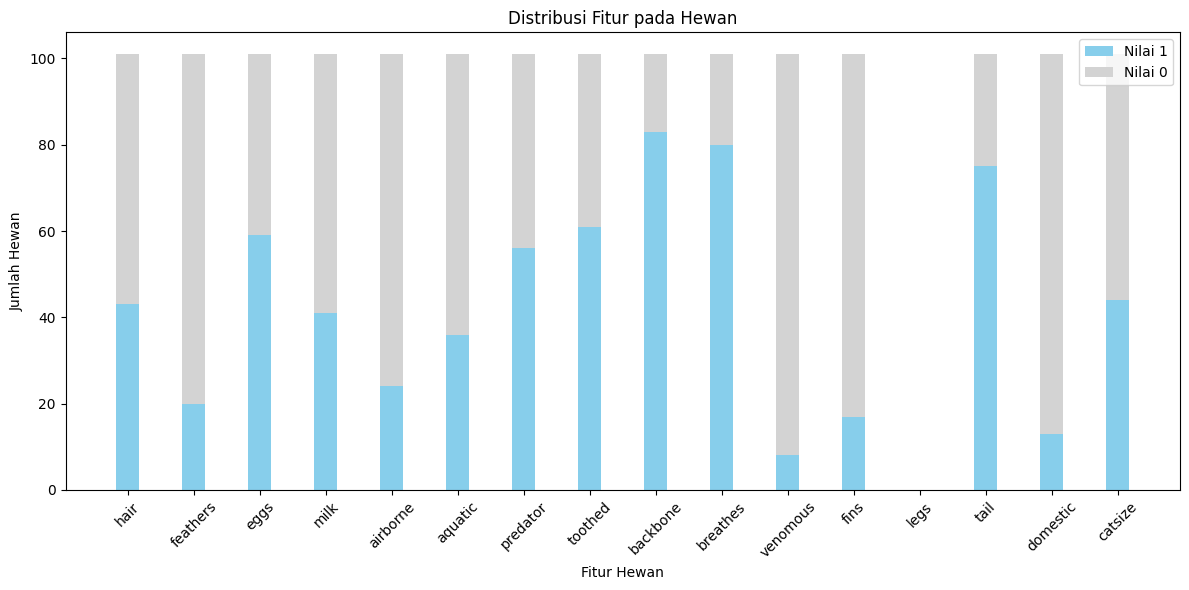
\includegraphics{Zoo0_files/figure-pdf/cell-10-output-1.png}

}

\end{figure}

Terlihat fitur yang mendominasi di tipe kategorikal terdapat pada
backbone atau hewan bertulang belakang sekitar 80, breathes atau hewan
yang bernafas sekitar 80 juga dan juga tail yaitu hewan yang memiliki
ekor sekitar 75 keatas

\hypertarget{rata-rata-distribusi-fitur-pada-keseluruhan-hewan-numerik}{%
\subsection{Rata rata distribusi fitur pada keseluruhan hewan
(Numerik)}\label{rata-rata-distribusi-fitur-pada-keseluruhan-hewan-numerik}}

\begin{Shaded}
\begin{Highlighting}[]
\CommentTok{\# Menghitung jumlah hewan dengan nilai legs tertentu}
\NormalTok{legs\_counts }\OperatorTok{=}\NormalTok{ df[}\StringTok{\textquotesingle{}legs\textquotesingle{}}\NormalTok{].value\_counts().sort\_index()}

\CommentTok{\# Membuat diagram garis untuk distribusi jumlah hewan berdasarkan jumlah kaki (legs)}
\NormalTok{plt.figure(figsize}\OperatorTok{=}\NormalTok{(}\DecValTok{8}\NormalTok{, }\DecValTok{6}\NormalTok{))}
\NormalTok{plt.plot(legs\_counts.index, legs\_counts.values, marker}\OperatorTok{=}\StringTok{\textquotesingle{}o\textquotesingle{}}\NormalTok{, color}\OperatorTok{=}\StringTok{\textquotesingle{}skyblue\textquotesingle{}}\NormalTok{, linestyle}\OperatorTok{=}\StringTok{\textquotesingle{}{-}\textquotesingle{}}\NormalTok{, linewidth}\OperatorTok{=}\DecValTok{2}\NormalTok{, markersize}\OperatorTok{=}\DecValTok{8}\NormalTok{)}
\NormalTok{plt.xlabel(}\StringTok{\textquotesingle{}Jumlah Kaki\textquotesingle{}}\NormalTok{)}
\NormalTok{plt.ylabel(}\StringTok{\textquotesingle{}Jumlah Hewan\textquotesingle{}}\NormalTok{)}
\NormalTok{plt.title(}\StringTok{\textquotesingle{}Distribusi Jumlah Kaki pada Hewan\textquotesingle{}}\NormalTok{)}
\NormalTok{plt.xticks(legs\_counts.index)}
\NormalTok{plt.grid(axis}\OperatorTok{=}\StringTok{\textquotesingle{}y\textquotesingle{}}\NormalTok{, linestyle}\OperatorTok{=}\StringTok{\textquotesingle{}{-}{-}\textquotesingle{}}\NormalTok{, alpha}\OperatorTok{=}\FloatTok{0.7}\NormalTok{)}

\CommentTok{\# Menambahkan label jumlah hewan pada setiap titik pada diagram}
\ControlFlowTok{for}\NormalTok{ i, count }\KeywordTok{in} \BuiltInTok{enumerate}\NormalTok{(legs\_counts.values):}
\NormalTok{    plt.text(legs\_counts.index[i], count, }\BuiltInTok{str}\NormalTok{(count), ha}\OperatorTok{=}\StringTok{\textquotesingle{}center\textquotesingle{}}\NormalTok{, va}\OperatorTok{=}\StringTok{\textquotesingle{}bottom\textquotesingle{}}\NormalTok{)}

\NormalTok{plt.tight\_layout()}
\NormalTok{plt.show()}
\end{Highlighting}
\end{Shaded}

\begin{figure}[H]

{\centering 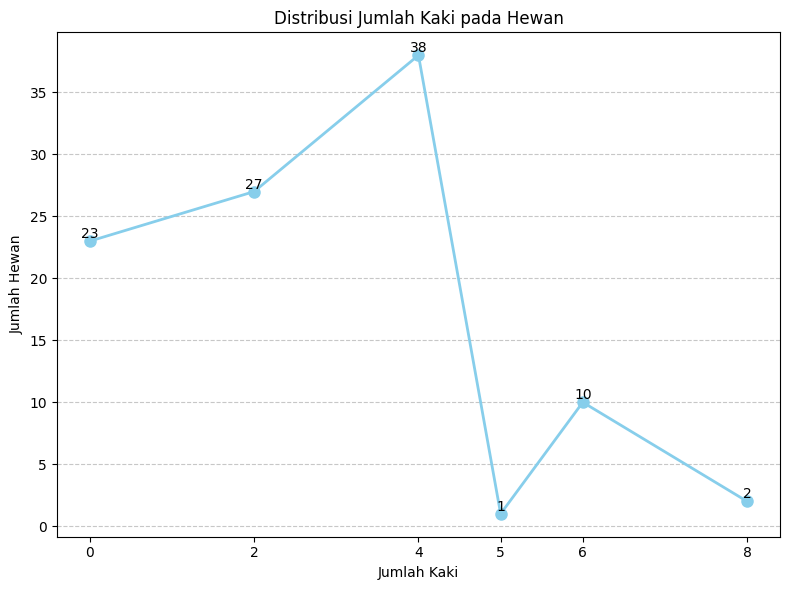
\includegraphics{Zoo0_files/figure-pdf/cell-11-output-1.png}

}

\end{figure}

Pada distribusi kaki ini, terlihat bahwa data dominan dengan hewan
berkaki 4 berjumlah 38 hewan dan data yang paling sedikit yaitu hewan
yang berkaki 5 yang hanya berjumlah 1

\hypertarget{distribusi-fitur-tanpa-kakilegs}{%
\subsection{Distribusi Fitur tanpa
kaki/legs}\label{distribusi-fitur-tanpa-kakilegs}}

Melihat fitur yang ada pada setiap \textbf{tipe} hewan tanpa label
legs(Numerik)

\begin{Shaded}
\begin{Highlighting}[]
\ImportTok{import}\NormalTok{ numpy }\ImportTok{as}\NormalTok{ np}
\ImportTok{import}\NormalTok{ matplotlib.pyplot }\ImportTok{as}\NormalTok{ plt}

\CommentTok{\# Menghitung jumlah tipe yang ada (1 sampai 7)}
\NormalTok{types }\OperatorTok{=}\NormalTok{ np.arange(}\DecValTok{1}\NormalTok{, }\DecValTok{8}\NormalTok{)}

\CommentTok{\# Dictionary untuk mapping tipe ke nama}
\NormalTok{tipe\_to\_nama }\OperatorTok{=}\NormalTok{ \{}
    \DecValTok{1}\NormalTok{: }\StringTok{"Mamalia"}\NormalTok{,}
    \DecValTok{2}\NormalTok{: }\StringTok{"Burung/Unggas"}\NormalTok{,}
    \DecValTok{3}\NormalTok{: }\StringTok{"Reptil"}\NormalTok{,}
    \DecValTok{4}\NormalTok{: }\StringTok{"Ikan"}\NormalTok{,}
    \DecValTok{5}\NormalTok{: }\StringTok{"Amfibi"}\NormalTok{,}
    \DecValTok{6}\NormalTok{: }\StringTok{"Serangga"}\NormalTok{,}
    \DecValTok{7}\NormalTok{: }\StringTok{"Moluska/Binatang Laut"}
\NormalTok{\}}

\CommentTok{\# Melakukan perulangan untuk setiap tipe}
\ControlFlowTok{for}\NormalTok{ tipe }\KeywordTok{in}\NormalTok{ types:}
    \CommentTok{\# Memfilter hanya baris dengan tipe tertentu}
\NormalTok{    filtered\_data }\OperatorTok{=}\NormalTok{ df[df[}\StringTok{\textquotesingle{}type\textquotesingle{}}\NormalTok{] }\OperatorTok{==}\NormalTok{ tipe]}

    \CommentTok{\# Menghitung jumlah hewan dalam tipe tersebut}
\NormalTok{    jumlah\_hewan }\OperatorTok{=} \BuiltInTok{len}\NormalTok{(filtered\_data)}

    \CommentTok{\# Menghitung jumlah hewan dalam tipe tersebut yang memiliki nilai setiap fitur}
\NormalTok{    fitur\_counts }\OperatorTok{=}\NormalTok{ filtered\_data.drop(columns}\OperatorTok{=}\NormalTok{[}\StringTok{\textquotesingle{}type\textquotesingle{}}\NormalTok{, }\StringTok{\textquotesingle{}animal\_name\textquotesingle{}}\NormalTok{, }\StringTok{\textquotesingle{}legs\textquotesingle{}}\NormalTok{]).}\BuiltInTok{apply}\NormalTok{(}\KeywordTok{lambda}\NormalTok{ x: x.value\_counts()).T}

    \CommentTok{\# Membuat diagram batang}
\NormalTok{    plt.figure(figsize}\OperatorTok{=}\NormalTok{(}\DecValTok{12}\NormalTok{, }\DecValTok{6}\NormalTok{))}
\NormalTok{    bar\_width }\OperatorTok{=} \FloatTok{0.35}
\NormalTok{    bar\_colors }\OperatorTok{=}\NormalTok{ [}\StringTok{\textquotesingle{}skyblue\textquotesingle{}}\NormalTok{] }\OperatorTok{*} \BuiltInTok{len}\NormalTok{(fitur\_counts.index)  }\CommentTok{\# Menggunakan warna sky blue untuk semua batang}
\NormalTok{    bar\_positions }\OperatorTok{=}\NormalTok{ np.arange(}\BuiltInTok{len}\NormalTok{(fitur\_counts.index))}

\NormalTok{    plt.bar(bar\_positions, fitur\_counts[}\DecValTok{1}\NormalTok{], bar\_width, color}\OperatorTok{=}\NormalTok{bar\_colors, label}\OperatorTok{=}\StringTok{\textquotesingle{}Nilai 1\textquotesingle{}}\NormalTok{)}
\NormalTok{    plt.bar(bar\_positions, fitur\_counts[}\DecValTok{0}\NormalTok{], bar\_width, color}\OperatorTok{=}\StringTok{\textquotesingle{}lightgray\textquotesingle{}}\NormalTok{, label}\OperatorTok{=}\StringTok{\textquotesingle{}Nilai 0\textquotesingle{}}\NormalTok{, bottom}\OperatorTok{=}\NormalTok{fitur\_counts[}\DecValTok{1}\NormalTok{])}

\NormalTok{    plt.xlabel(}\StringTok{\textquotesingle{}Nama Fitur\textquotesingle{}}\NormalTok{)}
\NormalTok{    plt.ylabel(}\StringTok{\textquotesingle{}Jumlah Hewan\textquotesingle{}}\NormalTok{)}
\NormalTok{    plt.title(}\SpecialStringTok{f\textquotesingle{}Distribusi Fitur pada Hewan dengan Tipe }\SpecialCharTok{\{}\NormalTok{tipe}\SpecialCharTok{\}}\SpecialStringTok{ (}\SpecialCharTok{\{}\NormalTok{tipe\_to\_nama[tipe]}\SpecialCharTok{\}}\SpecialStringTok{) {-} Jumlah Hewan: }\SpecialCharTok{\{}\NormalTok{jumlah\_hewan}\SpecialCharTok{\}}\SpecialStringTok{\textquotesingle{}}\NormalTok{)  }\CommentTok{\# Menambahkan jumlah hewan pada judul}
\NormalTok{    plt.xticks(bar\_positions, fitur\_counts.index, rotation}\OperatorTok{=}\DecValTok{45}\NormalTok{)}
\NormalTok{    plt.legend()}
\NormalTok{    plt.tight\_layout()}
\NormalTok{    plt.show()}
\end{Highlighting}
\end{Shaded}

\begin{figure}[H]

{\centering 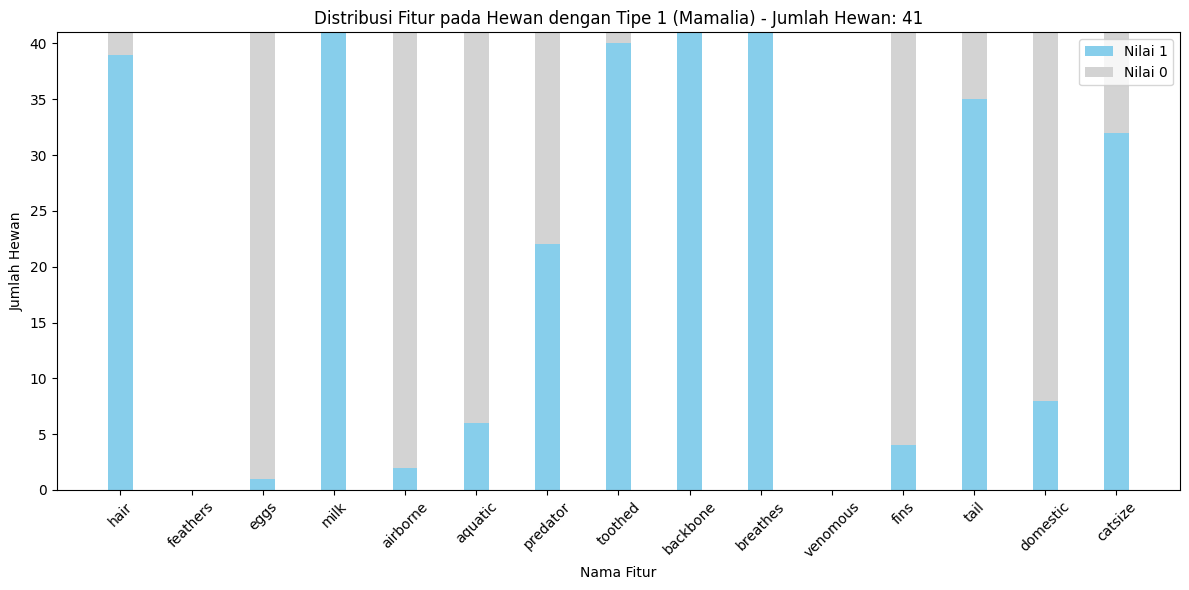
\includegraphics{Zoo0_files/figure-pdf/cell-12-output-1.png}

}

\end{figure}

\begin{figure}[H]

{\centering 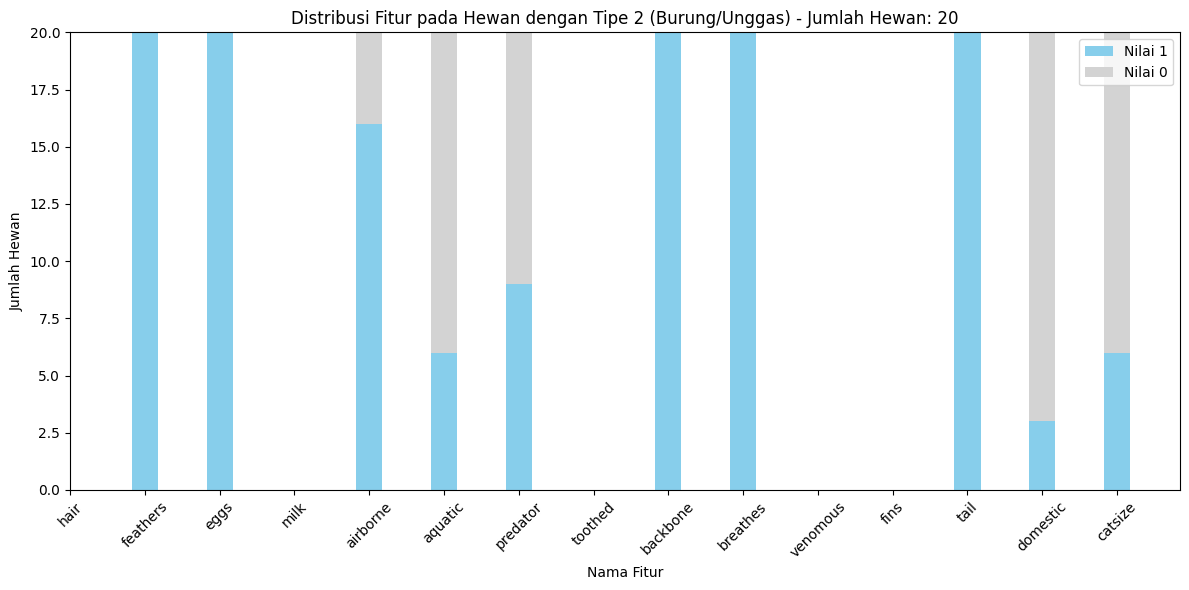
\includegraphics{Zoo0_files/figure-pdf/cell-12-output-2.png}

}

\end{figure}

\begin{figure}[H]

{\centering 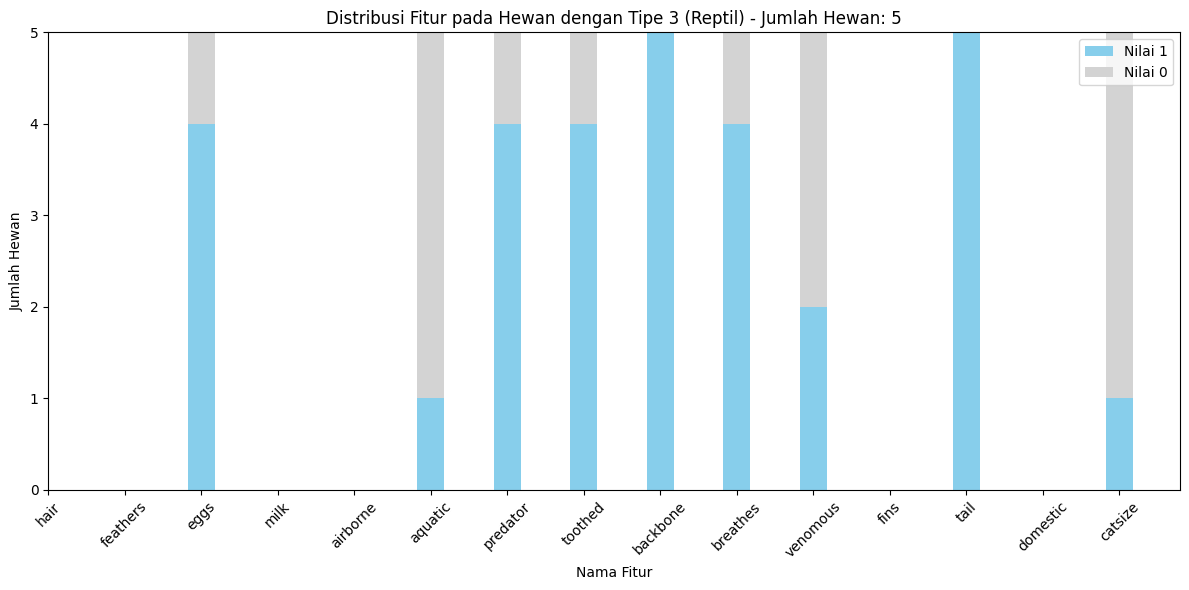
\includegraphics{Zoo0_files/figure-pdf/cell-12-output-3.png}

}

\end{figure}

\begin{figure}[H]

{\centering 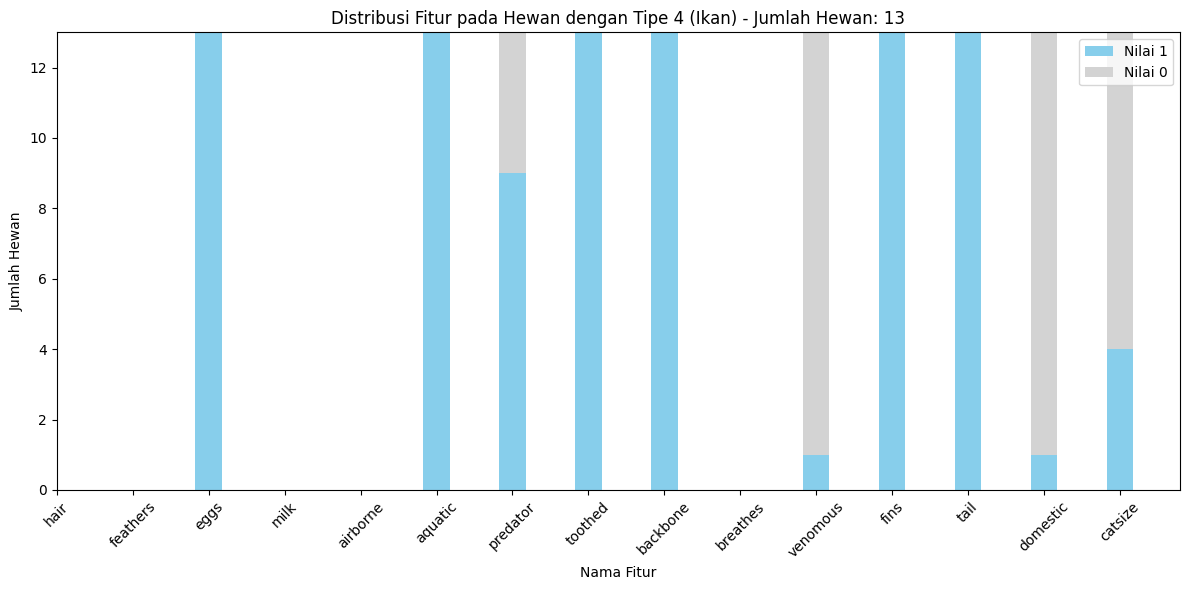
\includegraphics{Zoo0_files/figure-pdf/cell-12-output-4.png}

}

\end{figure}

\begin{figure}[H]

{\centering 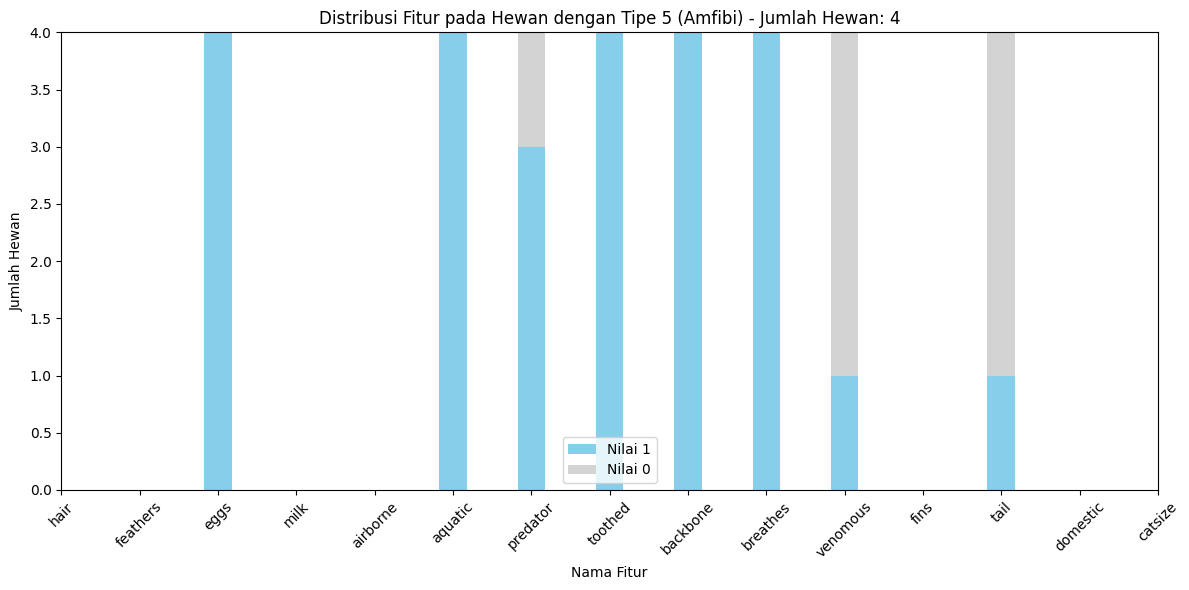
\includegraphics{Zoo0_files/figure-pdf/cell-12-output-5.png}

}

\end{figure}

\begin{figure}[H]

{\centering 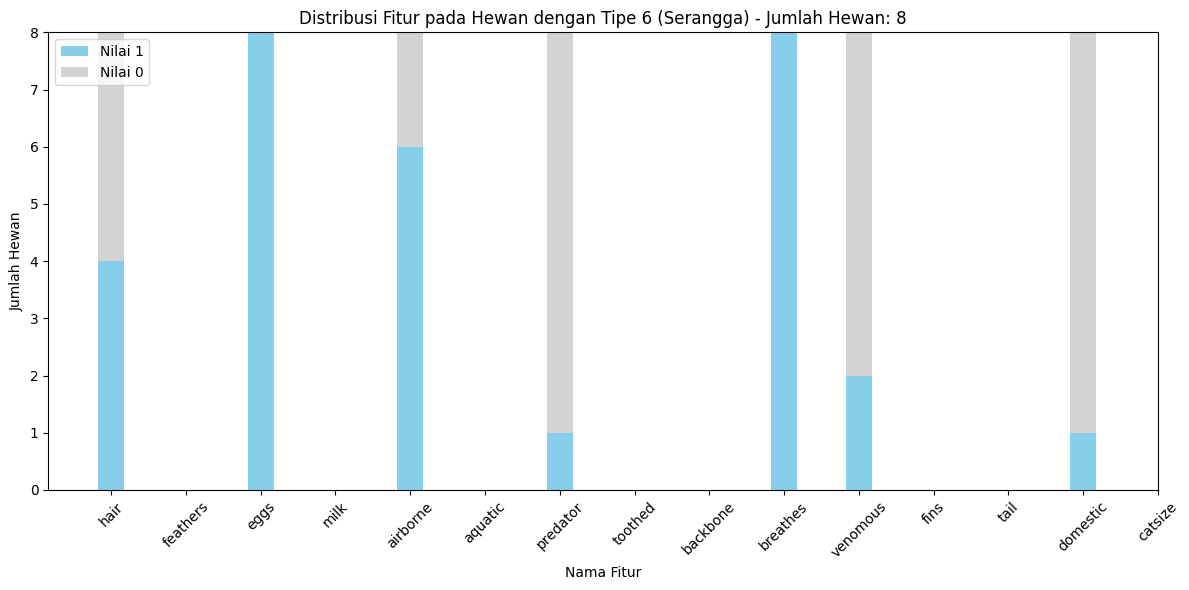
\includegraphics{Zoo0_files/figure-pdf/cell-12-output-6.png}

}

\end{figure}

\begin{figure}[H]

{\centering 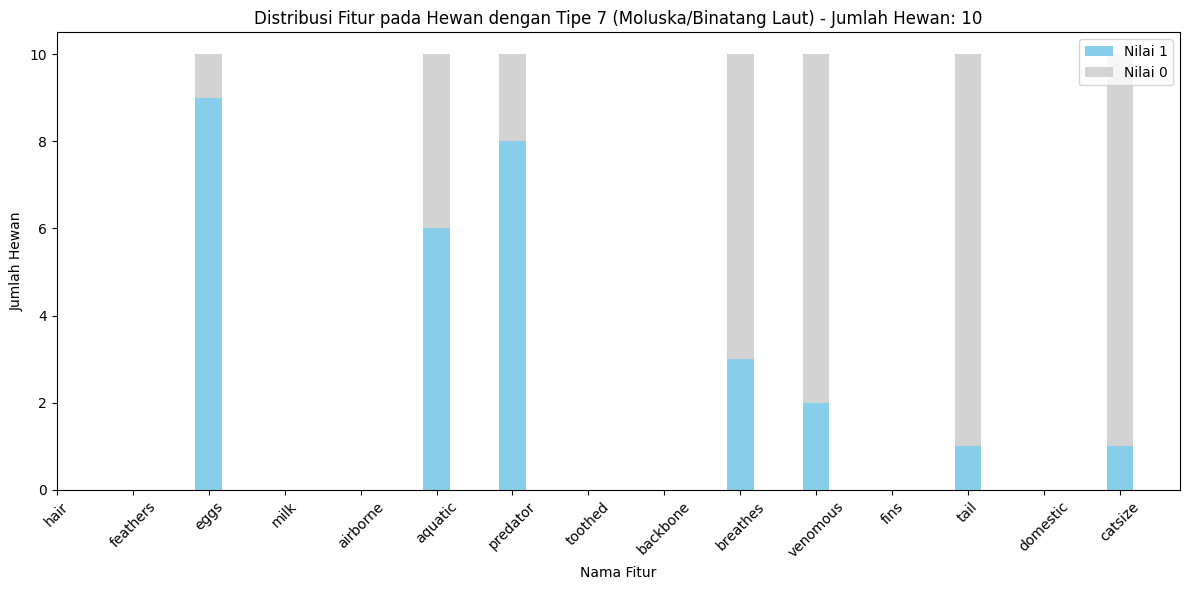
\includegraphics{Zoo0_files/figure-pdf/cell-12-output-7.png}

}

\end{figure}

Sedikit kesimpulan yang dapat diambil dari grafik diatas setiap tipe *
Tipe 1 : Hewan mamalia didominasi dengan 3 data tertinggi bahwa mereka
bernafas, memiliki tulang belakang, dan menyusui

\begin{itemize}
\item
  Tipe 2 : Hewan unggas/burung yang didominasi dengan 5 data tertinggi
  yaitu mereka berbulu, bertelur, bertulang belakang, bernafas, dan
  memiliki ekor
\item
  Tipe 3 : Hewan reptil yang didominasi dengan 2 data tertinggi yaitu
  bertulang belakang dan memiliki ekor
\item
  Tipe 4 : Hewan dengan tipe ikan yang didominasi dengan 6 data
  tertinggi yaitu mereka bertelur, hidup di air, bergigi, bertulang
  belakang, bersirip dan memiliki ekor
\item
  Tipe 5 : Hewan Amfibi memiliki 5 dominasi data tertinggi yaitu mereka
  bertelur, hidup di air, bergigi, bertulang belakang dan bernafas
\item
  Tipe 6 : Hewan serangga memiliki 2 dominasi data tertinggi yaitu
  mereka bertelur dan bernafas
\item
  Tipe 7 : Hewan moluska tidak memiliki data yang dimiliki oleh semua
  hewan di tipe tersebut namun ada data yang tinggi seperti mereka
  bertelur.
\end{itemize}

\hypertarget{distribusi-fitur-kaki}{%
\subsection{Distribusi fitur kaki}\label{distribusi-fitur-kaki}}

\begin{Shaded}
\begin{Highlighting}[]

\CommentTok{\# Menghitung jumlah tipe yang ada (1 sampai 7)}
\NormalTok{types }\OperatorTok{=}\NormalTok{ np.arange(}\DecValTok{1}\NormalTok{, }\DecValTok{8}\NormalTok{)}

\CommentTok{\# Dictionary untuk mapping tipe ke nama}
\NormalTok{tipe\_to\_nama }\OperatorTok{=}\NormalTok{ \{}
    \DecValTok{1}\NormalTok{: }\StringTok{"Mamalia"}\NormalTok{,}
    \DecValTok{2}\NormalTok{: }\StringTok{"Burung/Unggas"}\NormalTok{,}
    \DecValTok{3}\NormalTok{: }\StringTok{"Reptil"}\NormalTok{,}
    \DecValTok{4}\NormalTok{: }\StringTok{"Ikan"}\NormalTok{,}
    \DecValTok{5}\NormalTok{: }\StringTok{"Amfibi"}\NormalTok{,}
    \DecValTok{6}\NormalTok{: }\StringTok{"Serangga"}\NormalTok{,}
    \DecValTok{7}\NormalTok{: }\StringTok{"Moluska/Binatang Laut"}
\NormalTok{\}}

\CommentTok{\# Melakukan perulangan untuk setiap tipe}
\ControlFlowTok{for}\NormalTok{ tipe }\KeywordTok{in}\NormalTok{ types:}
    \CommentTok{\# Memfilter hanya baris dengan tipe tertentu}
\NormalTok{    filtered\_data }\OperatorTok{=}\NormalTok{ df[df[}\StringTok{\textquotesingle{}type\textquotesingle{}}\NormalTok{] }\OperatorTok{==}\NormalTok{ tipe]}

    \CommentTok{\# Menghitung jumlah hewan dalam tipe tersebut yang memiliki nilai 2, 4, 6, atau 8 kaki}
\NormalTok{    legs\_counts }\OperatorTok{=}\NormalTok{ filtered\_data[}\StringTok{\textquotesingle{}legs\textquotesingle{}}\NormalTok{].value\_counts().sort\_index()}

    \CommentTok{\# Membuat diagram batang untuk fitur \textquotesingle{}legs\textquotesingle{} pada tipe tersebut}
\NormalTok{    plt.figure(figsize}\OperatorTok{=}\NormalTok{(}\DecValTok{8}\NormalTok{, }\DecValTok{6}\NormalTok{))}
\NormalTok{    bar\_positions }\OperatorTok{=}\NormalTok{ np.arange(}\BuiltInTok{len}\NormalTok{(legs\_counts.index))}
\NormalTok{    bar\_colors }\OperatorTok{=}\NormalTok{ [}\StringTok{\textquotesingle{}skyblue\textquotesingle{}}\NormalTok{] }\OperatorTok{*} \BuiltInTok{len}\NormalTok{(legs\_counts.index)  }\CommentTok{\# Menggunakan warna sky blue untuk semua batang}

\NormalTok{    plt.bar(bar\_positions, legs\_counts, color}\OperatorTok{=}\NormalTok{bar\_colors, edgecolor}\OperatorTok{=}\StringTok{\textquotesingle{}black\textquotesingle{}}\NormalTok{)}
\NormalTok{    plt.xlabel(}\StringTok{\textquotesingle{}Jumlah Kaki\textquotesingle{}}\NormalTok{)}
\NormalTok{    plt.ylabel(}\StringTok{\textquotesingle{}Jumlah Hewan\textquotesingle{}}\NormalTok{)}
\NormalTok{    plt.title(}\SpecialStringTok{f\textquotesingle{}Distribusi Jumlah Kaki pada Hewan dengan Tipe }\SpecialCharTok{\{}\NormalTok{tipe}\SpecialCharTok{\}}\SpecialStringTok{ (}\SpecialCharTok{\{}\NormalTok{tipe\_to\_nama[tipe]}\SpecialCharTok{\}}\SpecialStringTok{)\textquotesingle{}}\NormalTok{)  }\CommentTok{\# Menambahkan nama tipe}
\NormalTok{    plt.xticks(bar\_positions, legs\_counts.index)}
\NormalTok{    plt.grid(axis}\OperatorTok{=}\StringTok{\textquotesingle{}y\textquotesingle{}}\NormalTok{, linestyle}\OperatorTok{=}\StringTok{\textquotesingle{}{-}{-}\textquotesingle{}}\NormalTok{, alpha}\OperatorTok{=}\FloatTok{0.7}\NormalTok{)}
\NormalTok{    plt.tight\_layout()}
\NormalTok{    plt.show()}
\end{Highlighting}
\end{Shaded}

\begin{figure}[H]

{\centering 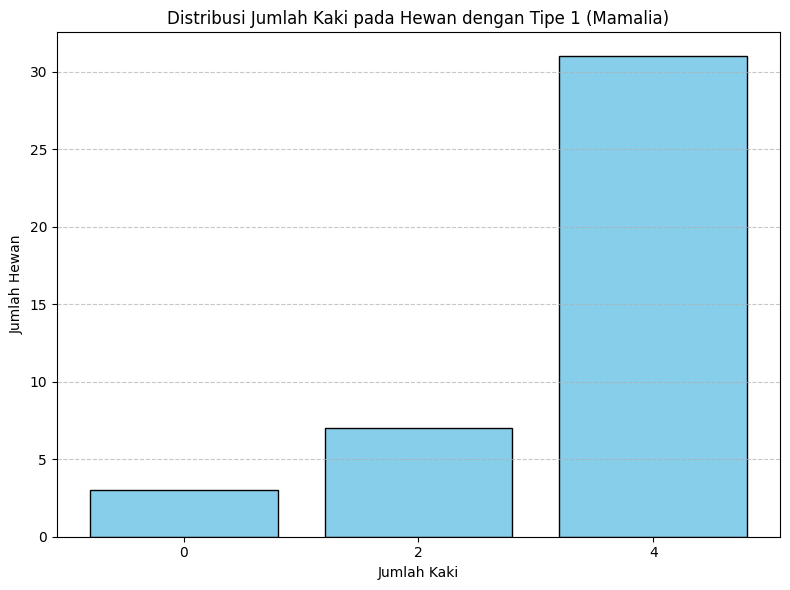
\includegraphics{Zoo0_files/figure-pdf/cell-13-output-1.png}

}

\end{figure}

\begin{figure}[H]

{\centering 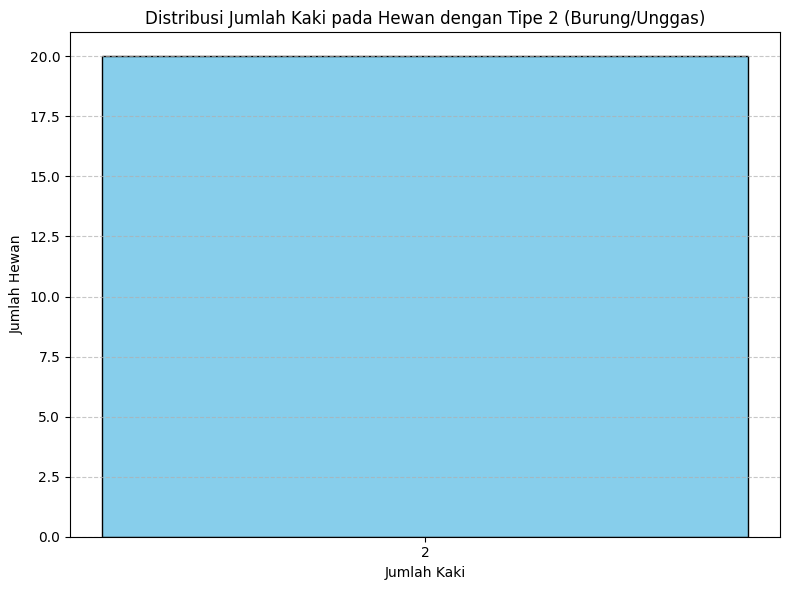
\includegraphics{Zoo0_files/figure-pdf/cell-13-output-2.png}

}

\end{figure}

\begin{figure}[H]

{\centering 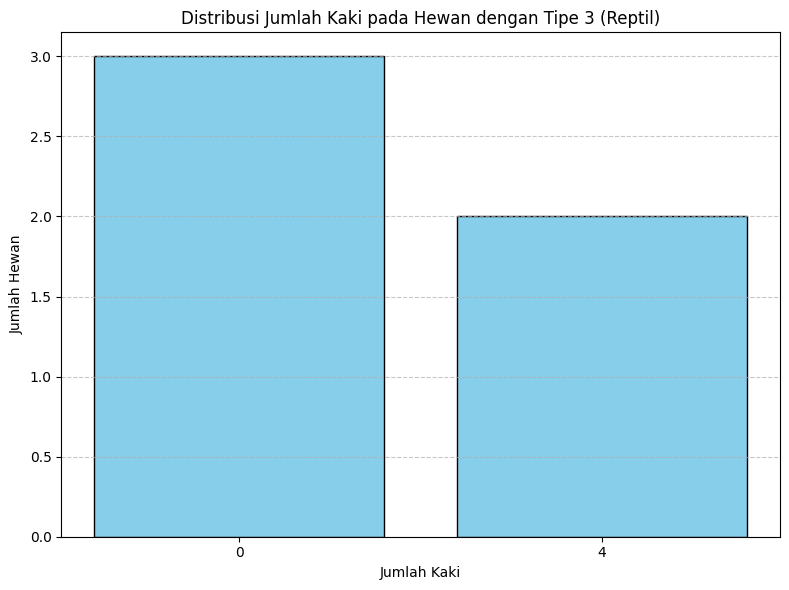
\includegraphics{Zoo0_files/figure-pdf/cell-13-output-3.png}

}

\end{figure}

\begin{figure}[H]

{\centering 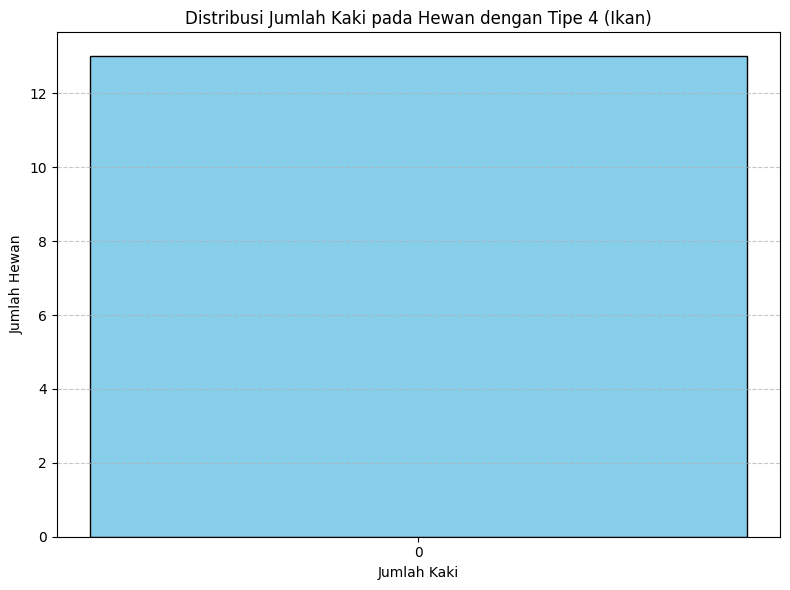
\includegraphics{Zoo0_files/figure-pdf/cell-13-output-4.png}

}

\end{figure}

\begin{figure}[H]

{\centering 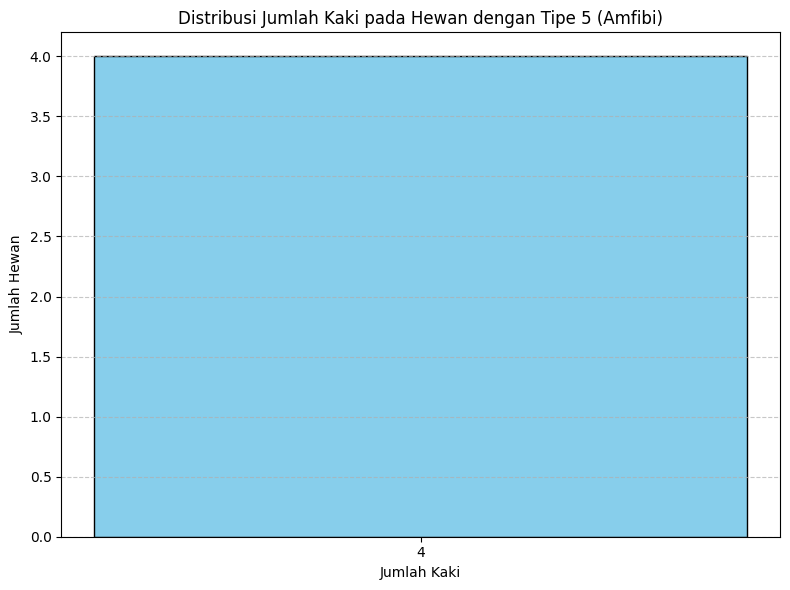
\includegraphics{Zoo0_files/figure-pdf/cell-13-output-5.png}

}

\end{figure}

\begin{figure}[H]

{\centering 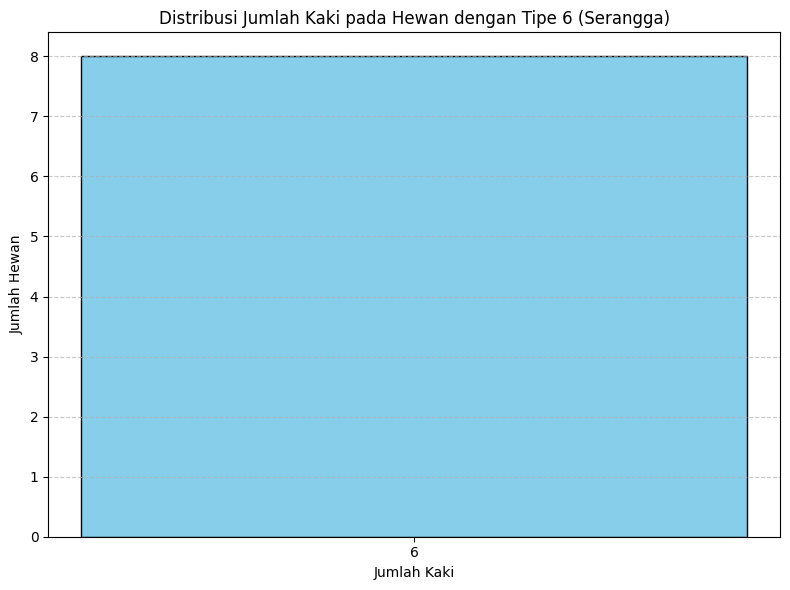
\includegraphics{Zoo0_files/figure-pdf/cell-13-output-6.png}

}

\end{figure}

\begin{figure}[H]

{\centering 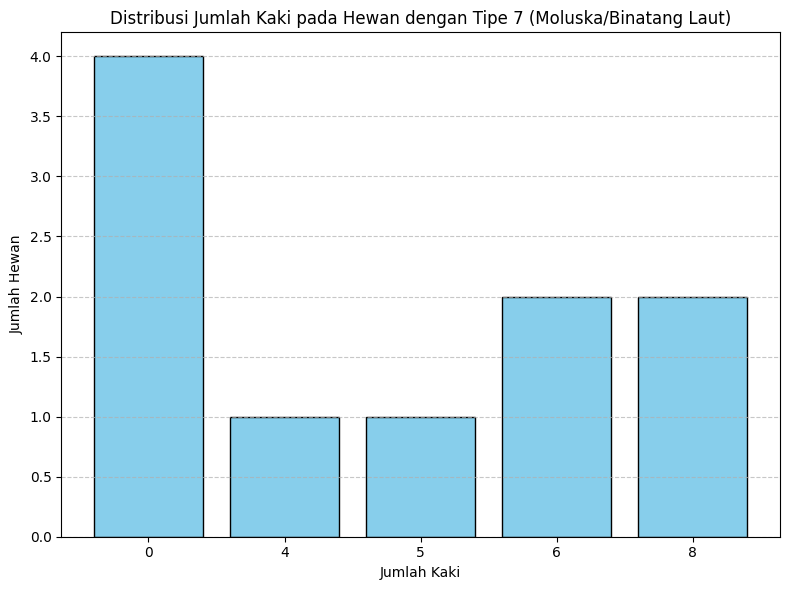
\includegraphics{Zoo0_files/figure-pdf/cell-13-output-7.png}

}

\end{figure}

\begin{itemize}
\tightlist
\item
  Tipe 1 : Hewan mamalia ada yang tidak memiliki kaki, ada yang 2 kaki,
  lalu ada yang 4 kaki
\item
  Tipe 2 : Burung/Unggas rata dengan kaki berjumlah 2
\item
  Tipe 3 : Reptil ada yang tidak memiliki kaki lalu ada yang memiliki 4
  kaki
\item
  Tipe 4 : Ikan tidak ada yang memiliki kaki
\item
  Tipe 5 : Amfibi memiliki 4 jumlah kaki
\item
  Tipe 6 : Serangga memiliki 6 kaki
\item
  Tipe 7 : Moluska / binatang laut memiliki kaki yang beragam seperti
  ada yang tidak memiliki kaki, ada yang berkaki 4, 5, 6, dan 8
\end{itemize}

\hypertarget{pengurutan-nama-hewan-berdasarkan-kaki}{%
\subsection{Pengurutan nama Hewan berdasarkan
kaki}\label{pengurutan-nama-hewan-berdasarkan-kaki}}

Kode yang ada dibawah ini dibuat agar bisa mengetahui apa saja hewan
yang terlibat dalam pengenalan dataset hewan apa saja yang punya kaki
atau tidak.

\begin{Shaded}
\begin{Highlighting}[]
\CommentTok{\# Menghitung jumlah tipe yang ada (1 sampai 7)}
\NormalTok{types }\OperatorTok{=}\NormalTok{ np.arange(}\DecValTok{1}\NormalTok{, }\DecValTok{8}\NormalTok{)}

\CommentTok{\# Dictionary untuk mapping tipe ke nama}
\NormalTok{tipe\_to\_nama }\OperatorTok{=}\NormalTok{ \{}
    \DecValTok{1}\NormalTok{: }\StringTok{"Mamalia"}\NormalTok{,}
    \DecValTok{2}\NormalTok{: }\StringTok{"Burung/Unggas"}\NormalTok{,}
    \DecValTok{3}\NormalTok{: }\StringTok{"Reptil"}\NormalTok{,}
    \DecValTok{4}\NormalTok{: }\StringTok{"Ikan"}\NormalTok{,}
    \DecValTok{5}\NormalTok{: }\StringTok{"Amfibi"}\NormalTok{,}
    \DecValTok{6}\NormalTok{: }\StringTok{"Serangga"}\NormalTok{,}
    \DecValTok{7}\NormalTok{: }\StringTok{"Moluska/Binatang Laut"}
\NormalTok{\}}

\CommentTok{\# Melakukan perulangan untuk setiap tipe}
\ControlFlowTok{for}\NormalTok{ tipe }\KeywordTok{in}\NormalTok{ types:}
    \CommentTok{\# Memfilter hanya baris dengan tipe tertentu}
\NormalTok{    filtered\_data }\OperatorTok{=}\NormalTok{ df[df[}\StringTok{\textquotesingle{}type\textquotesingle{}}\NormalTok{] }\OperatorTok{==}\NormalTok{ tipe]}

    \CommentTok{\# Mengelompokkan data berdasarkan jumlah kaki (legs) pada tipe tersebut}
\NormalTok{    legs\_groups }\OperatorTok{=}\NormalTok{ filtered\_data.groupby(}\StringTok{\textquotesingle{}legs\textquotesingle{}}\NormalTok{)[}\StringTok{\textquotesingle{}animal\_name\textquotesingle{}}\NormalTok{].}\BuiltInTok{apply}\NormalTok{(}\BuiltInTok{list}\NormalTok{)}

    \CommentTok{\# Menampilkan nama{-}nama binatang berdasarkan jumlah kaki}
    \BuiltInTok{print}\NormalTok{(}\SpecialStringTok{f"Tipe }\SpecialCharTok{\{}\NormalTok{tipe}\SpecialCharTok{\}}\SpecialStringTok{ (}\SpecialCharTok{\{}\NormalTok{tipe\_to\_nama[tipe]}\SpecialCharTok{\}}\SpecialStringTok{)"}\NormalTok{)}
    \ControlFlowTok{for}\NormalTok{ legs, animals }\KeywordTok{in}\NormalTok{ legs\_groups.items():}
        \BuiltInTok{print}\NormalTok{(}\SpecialStringTok{f"Jumlah Kaki: }\SpecialCharTok{\{}\NormalTok{legs}\SpecialCharTok{\}}\SpecialStringTok{"}\NormalTok{)}
        \BuiltInTok{print}\NormalTok{(}\SpecialStringTok{f"Binatang: }\SpecialCharTok{\{}\StringTok{\textquotesingle{}, \textquotesingle{}}\SpecialCharTok{.}\NormalTok{join(animals)}\SpecialCharTok{\}}\SpecialStringTok{"}\NormalTok{)}
        \BuiltInTok{print}\NormalTok{(}\StringTok{"="}\OperatorTok{*}\DecValTok{30}\NormalTok{)}
    \BuiltInTok{print}\NormalTok{(}\StringTok{"}\CharTok{\textbackslash{}n}\StringTok{"}\NormalTok{)}
\end{Highlighting}
\end{Shaded}

\begin{verbatim}
Tipe 1 (Mamalia)
Jumlah Kaki: 0
Binatang: dolphin, porpoise, seal
==============================
Jumlah Kaki: 2
Binatang: fruitbat, girl, gorilla, sealion, squirrel, vampire, wallaby
==============================
Jumlah Kaki: 4
Binatang: aardvark, antelope, bear, boar, buffalo, calf, cavy, cheetah, deer, elephant, giraffe, goat, hamster, hare, leopard, lion, lynx, mink, mole, mongoose, opossum, oryx, platypus, polecat, pony, puma, pussycat, raccoon, reindeer, vole, wolf
==============================


Tipe 2 (Burung/Unggas)
Jumlah Kaki: 2
Binatang: chicken, crow, dove, duck, flamingo, gull, hawk, kiwi, lark, ostrich, parakeet, penguin, pheasant, rhea, skimmer, skua, sparrow, swan, vulture, wren
==============================


Tipe 3 (Reptil)
Jumlah Kaki: 0
Binatang: pitviper, seasnake, slowworm
==============================
Jumlah Kaki: 4
Binatang: tortoise, tuatara
==============================


Tipe 4 (Ikan)
Jumlah Kaki: 0
Binatang: bass, carp, catfish, chub, dogfish, haddock, herring, pike, piranha, seahorse, sole, stingray, tuna
==============================


Tipe 5 (Amfibi)
Jumlah Kaki: 4
Binatang: frog, frog, newt, toad
==============================


Tipe 6 (Serangga)
Jumlah Kaki: 6
Binatang: flea, gnat, honeybee, housefly, ladybird, moth, termite, wasp
==============================


Tipe 7 (Moluska/Binatang Laut)
Jumlah Kaki: 0
Binatang: clam, seawasp, slug, worm
==============================
Jumlah Kaki: 4
Binatang: crab
==============================
Jumlah Kaki: 5
Binatang: starfish
==============================
Jumlah Kaki: 6
Binatang: crayfish, lobster
==============================
Jumlah Kaki: 8
Binatang: octopus, scorpion
==============================

\end{verbatim}

\hypertarget{missing-value}{%
\subsection{Missing value}\label{missing-value}}

Cek apakah ada missing value pada dataset

\begin{Shaded}
\begin{Highlighting}[]
\BuiltInTok{print}\NormalTok{(X.isnull().}\BuiltInTok{sum}\NormalTok{())  }\CommentTok{\# Menampilkan jumlah missing value untuk setiap kolom}
\end{Highlighting}
\end{Shaded}

\begin{verbatim}
hair        0
feathers    0
eggs        0
milk        0
airborne    0
aquatic     0
predator    0
toothed     0
backbone    0
breathes    0
venomous    0
fins        0
legs        0
tail        0
domestic    0
catsize     0
dtype: int64
\end{verbatim}

\begin{center}\rule{0.5\linewidth}{0.5pt}\end{center}

\hypertarget{split-data}{%
\subsection{Split data}\label{split-data}}

\begin{Shaded}
\begin{Highlighting}[]
\ImportTok{from}\NormalTok{ sklearn.model\_selection }\ImportTok{import}\NormalTok{ train\_test\_split}


\CommentTok{\# Pembagian data menjadi data latih dan data uji (80\% data latih, 20\% data uji)}
\NormalTok{X\_train, X\_test, y\_train, y\_test }\OperatorTok{=}\NormalTok{ train\_test\_split(X, y, test\_size}\OperatorTok{=}\FloatTok{0.2}\NormalTok{, random\_state}\OperatorTok{=}\DecValTok{42}\NormalTok{)}
\end{Highlighting}
\end{Shaded}

Data setelah di split tapi belum di Smote

\begin{Shaded}
\begin{Highlighting}[]
\NormalTok{X\_train.shape}
\end{Highlighting}
\end{Shaded}

\begin{verbatim}
(80, 16)
\end{verbatim}

\begin{Shaded}
\begin{Highlighting}[]
\NormalTok{y\_train}
\end{Highlighting}
\end{Shaded}

\begin{verbatim}
89    5
26    5
42    6
70    1
15    7
     ..
60    4
71    2
14    7
92    4
51    6
Name: type, Length: 80, dtype: int64
\end{verbatim}

\hypertarget{smote}{%
\subsection{Smote}\label{smote}}

Smote atau Synthetic Minority Over-sampling Technique yaitu metode
oversampling yang digunakan untuk menangani ketidakseimbangan kelas
dalam masalah klasifikasi. Pada dataset Zoo dilakukan SMOTE karena
datanya yang tidak balance dan dapat dilihat pada visualisasi dibawah
sebagai perbandingan data yang tidak balance atau sebelum di SMOTE
dengan data yang sudah di SMOTE sehingga menjadi balance

\begin{Shaded}
\begin{Highlighting}[]
\ImportTok{from}\NormalTok{ imblearn.over\_sampling }\ImportTok{import}\NormalTok{ SMOTE}
\CommentTok{\# smote data untuk memberi data sintetis}
\NormalTok{smote }\OperatorTok{=}\NormalTok{ SMOTE(random\_state}\OperatorTok{=}\DecValTok{42}\NormalTok{,k\_neighbors}\OperatorTok{=}\DecValTok{3}\NormalTok{)}
\NormalTok{X\_train\_resampled, y\_train\_resampled }\OperatorTok{=}\NormalTok{ smote.fit\_resample(X\_train, y\_train)}
\end{Highlighting}
\end{Shaded}

\begin{Shaded}
\begin{Highlighting}[]
\NormalTok{X\_train\_resampled.shape}
\end{Highlighting}
\end{Shaded}

\begin{verbatim}
(203, 16)
\end{verbatim}

\begin{Shaded}
\begin{Highlighting}[]
\NormalTok{y\_train\_resampled.shape}
\end{Highlighting}
\end{Shaded}

\begin{verbatim}
(203,)
\end{verbatim}

\hypertarget{visualisasi}{%
\subsection{Visualisasi}\label{visualisasi}}

\begin{Shaded}
\begin{Highlighting}[]
\ImportTok{import}\NormalTok{ matplotlib.pyplot }\ImportTok{as}\NormalTok{ plt}

\CommentTok{\# Menghitung jumlah tipe yang ada pada y\_train sebelum dan setelah SMOTE}
\NormalTok{unique\_classes\_original }\OperatorTok{=}\NormalTok{ y\_train.value\_counts().sort\_index()}
\NormalTok{unique\_classes\_resampled }\OperatorTok{=}\NormalTok{ y\_train\_resampled.value\_counts().sort\_index()}

\CommentTok{\# Mengatur posisi bar pada diagram histogram}
\NormalTok{bar\_positions\_original }\OperatorTok{=} \BuiltInTok{range}\NormalTok{(}\BuiltInTok{len}\NormalTok{(unique\_classes\_original))}
\NormalTok{bar\_positions\_resampled }\OperatorTok{=}\NormalTok{ [pos }\OperatorTok{+} \FloatTok{0.4} \ControlFlowTok{for}\NormalTok{ pos }\KeywordTok{in}\NormalTok{ bar\_positions\_original]}

\CommentTok{\# Membuat diagram histogram}
\NormalTok{plt.figure(figsize}\OperatorTok{=}\NormalTok{(}\DecValTok{8}\NormalTok{, }\DecValTok{6}\NormalTok{))}
\NormalTok{plt.bar(bar\_positions\_original, unique\_classes\_original, width}\OperatorTok{=}\FloatTok{0.4}\NormalTok{, label}\OperatorTok{=}\StringTok{\textquotesingle{}Sebelum SMOTE\textquotesingle{}}\NormalTok{, color}\OperatorTok{=}\StringTok{\textquotesingle{}skyblue\textquotesingle{}}\NormalTok{)}
\NormalTok{plt.bar(bar\_positions\_resampled, unique\_classes\_resampled, width}\OperatorTok{=}\FloatTok{0.4}\NormalTok{, label}\OperatorTok{=}\StringTok{\textquotesingle{}Setelah SMOTE\textquotesingle{}}\NormalTok{, color}\OperatorTok{=}\StringTok{\textquotesingle{}orange\textquotesingle{}}\NormalTok{)}

\CommentTok{\# Menyertakan label pada sumbu x dan y serta judul diagram}
\NormalTok{plt.xlabel(}\StringTok{\textquotesingle{}Tipe\textquotesingle{}}\NormalTok{)}
\NormalTok{plt.ylabel(}\StringTok{\textquotesingle{}Jumlah Hewan\textquotesingle{}}\NormalTok{)}
\NormalTok{plt.title(}\StringTok{\textquotesingle{}Distribusi Kelas Hewan Sebelum dan Setelah SMOTE\textquotesingle{}}\NormalTok{)}
\NormalTok{plt.xticks([pos }\OperatorTok{+} \FloatTok{0.2} \ControlFlowTok{for}\NormalTok{ pos }\KeywordTok{in}\NormalTok{ bar\_positions\_original], unique\_classes\_original.index)}
\NormalTok{plt.legend()}
\NormalTok{plt.tight\_layout()}
\NormalTok{plt.show()}
\end{Highlighting}
\end{Shaded}

\begin{figure}[H]

{\centering 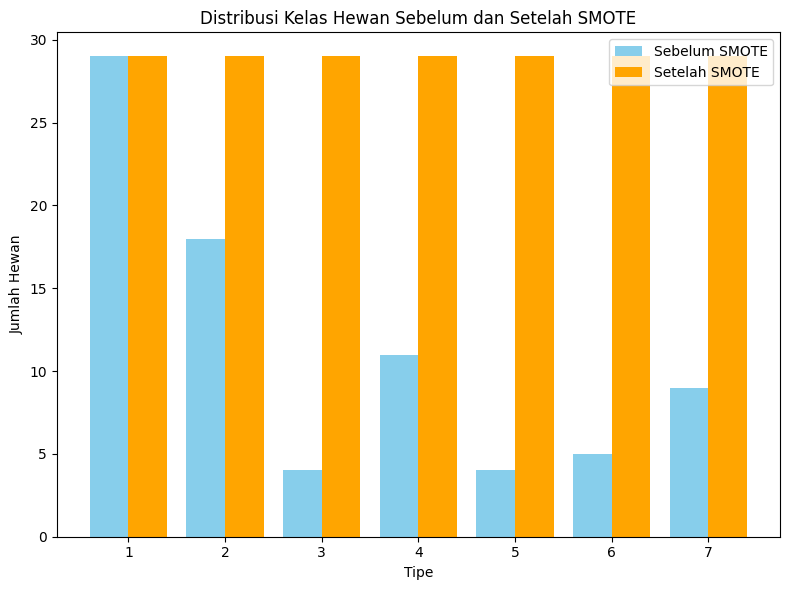
\includegraphics{Zoo0_files/figure-pdf/cell-22-output-1.png}

}

\end{figure}

Diagram batang biru merupakan data yang belum di balance sedangkan
diagram batang kuning merupakan data yang sudah balance.

\hypertarget{modelling}{%
\section{Modelling}\label{modelling}}

\hypertarget{random-forest}{%
\subsection{Random Forest}\label{random-forest}}

Rumus umum Random Forest
\[f(x) = \text{sign}\left(\frac{1}{N} \sum_{i=1}^{N} f_i(x) - \theta\right)
\] Dengan penjelasan:
\[\\\ N \text{ adalah jumlah pohon dalam hutan, } \\\ f_i(x) \text{ adalah prediksi dari pohon ke-} i,\\\ \text{ dan } \theta \text{ adalah ambang batas (threshold).}\]

\begin{Shaded}
\begin{Highlighting}[]
\ImportTok{from}\NormalTok{ sklearn.ensemble }\ImportTok{import}\NormalTok{ RandomForestClassifier}
\ImportTok{from}\NormalTok{ sklearn.metrics }\ImportTok{import}\NormalTok{ accuracy\_score, classification\_report}


\CommentTok{\# Membangun model Random Forest Classifier}
\NormalTok{rf\_clf }\OperatorTok{=}\NormalTok{ RandomForestClassifier(random\_state}\OperatorTok{=}\DecValTok{42}\NormalTok{)}
\NormalTok{rf\_clf.fit(X\_train\_resampled, y\_train\_resampled.values.ravel())}
\end{Highlighting}
\end{Shaded}

\begin{verbatim}
RandomForestClassifier(random_state=42)
\end{verbatim}

\hypertarget{support-vector-machine}{%
\subsection{Support Vector Machine}\label{support-vector-machine}}

Rumus umum pada SVM adalah

\[\text{SVM: } f(x) = \text{sign}\left(\sum_{i=1}^{N} \alpha_i y_i K(x, x_i) + b\right)\]
dengan penjelasan

\begin{align*}
f(x) & : \text{Fungsi keputusan SVM untuk input } x \\
\alpha_i & : \text{Bobot yang diberikan kepada sampel pelatihan ke-} i \\
y_i & : \text{Kelas dari sampel pelatihan ke-} i \\
K(x, x_i) & : \text{Fungsi kernel yang mengukur "kedekatan" antara } x \text{ dan } x_i \\
b & : \text{Bias atau penyesuaian}
\end{align*}

\begin{Shaded}
\begin{Highlighting}[]
\ImportTok{from}\NormalTok{ sklearn.svm }\ImportTok{import}\NormalTok{ SVC}
\ImportTok{from}\NormalTok{ sklearn.metrics }\ImportTok{import}\NormalTok{ accuracy\_score, classification\_report}
\CommentTok{\# Membangun model SVM untuk klasifikasi}
\NormalTok{svm\_clf }\OperatorTok{=}\NormalTok{ SVC(random\_state}\OperatorTok{=}\DecValTok{44}\NormalTok{)}
\NormalTok{svm\_clf.fit(X\_train\_resampled, y\_train\_resampled.values.ravel())}
\end{Highlighting}
\end{Shaded}

\begin{verbatim}
SVC(random_state=44)
\end{verbatim}

\hypertarget{decision-tree}{%
\subsection{Decision Tree}\label{decision-tree}}

Rumus umum Decision Tree: \[
f(x) = \text{sign}\left(\text{Node}(x) - \theta\right)
\] Dengan penjelasan: \[
\text{Node}(x):\text{Fungsi keputusan pohon keputusan untuk input } x
\\\ \theta: \text{ adalah ambang batas (threshold).}
\]

\begin{Shaded}
\begin{Highlighting}[]
\ImportTok{from}\NormalTok{ sklearn.tree }\ImportTok{import}\NormalTok{ DecisionTreeClassifier}
\ImportTok{from}\NormalTok{ sklearn.metrics }\ImportTok{import}\NormalTok{ accuracy\_score, classification\_report}

\CommentTok{\# Membangun model Decision Tree untuk klasifikasi}
\NormalTok{decision\_tree\_clf }\OperatorTok{=}\NormalTok{ DecisionTreeClassifier(random\_state}\OperatorTok{=}\DecValTok{42}\NormalTok{)}
\NormalTok{decision\_tree\_clf.fit(X\_train\_resampled, y\_train\_resampled.values.ravel())}
\end{Highlighting}
\end{Shaded}

\begin{verbatim}
DecisionTreeClassifier(random_state=42)
\end{verbatim}

\hypertarget{logistic-regresion}{%
\subsection{Logistic Regresion}\label{logistic-regresion}}

Rumus umum Logistic Regression: \[
f(x) = \frac{1}{1 + \exp(-\left(\sum_{i=1}^{N} w_i x_i + b\right))}
\] Dengan penjelasan: \[
\begin{align*}
f(x) & : \text{Fungsi keputusan Logistic Regression untuk input } x \\
w_i & : \text{Bobot input ke-} i \\
x_i & : \text{Input ke-} i \\
b & : \text{Bias}
\end{align*}
\]

\begin{Shaded}
\begin{Highlighting}[]
\ImportTok{from}\NormalTok{ sklearn.linear\_model }\ImportTok{import}\NormalTok{ LogisticRegression}
\ImportTok{from}\NormalTok{ sklearn.metrics }\ImportTok{import}\NormalTok{ accuracy\_score, classification\_report}

\CommentTok{\# Membangun model Logistic Regression untuk klasifikasi}
\NormalTok{logistic\_reg\_clf }\OperatorTok{=}\NormalTok{ LogisticRegression(random\_state}\OperatorTok{=}\DecValTok{42}\NormalTok{,max\_iter}\OperatorTok{=}\DecValTok{1000}\NormalTok{)}
\NormalTok{logistic\_reg\_clf.fit(X\_train\_resampled, y\_train\_resampled.values.ravel())}
\end{Highlighting}
\end{Shaded}

\begin{verbatim}
LogisticRegression(max_iter=1000, random_state=42)
\end{verbatim}

\hypertarget{neural-network}{%
\subsection{Neural Network}\label{neural-network}}

Rumus umum ANN: \[
f(x) = \text{sign}\left(\sum_{j=1}^{M} w_j g\left(\sum_{i=1}^{N} w_{ij} x_i + b_j\right) + b\right)
\] Dengan penjelasan: \[
\begin{align*}
f(x) & : \text{Fungsi keputusan ANN untuk input } x \\
w_j & : \text{Bobot output ke-} j \\
g(\cdot) & : \text{Fungsi aktivasi} \\
w_{ij} & : \text{Bobot input ke-} j \\
x_i & : \text{Input ke-} i \\
b_j & : \text{Bias ke-} j \\
b & : \text{Bias output}
\end{align*}
\]

\begin{Shaded}
\begin{Highlighting}[]
\ImportTok{from}\NormalTok{ sklearn.neural\_network }\ImportTok{import}\NormalTok{ MLPClassifier}
\ImportTok{from}\NormalTok{ sklearn.metrics }\ImportTok{import}\NormalTok{ accuracy\_score, classification\_report}

\CommentTok{\# Membangun model Neural Network untuk klasifikasi}
\NormalTok{ann\_clf }\OperatorTok{=}\NormalTok{ MLPClassifier(hidden\_layer\_sizes}\OperatorTok{=}\NormalTok{(}\DecValTok{512}\NormalTok{,}\DecValTok{256}\NormalTok{), max\_iter}\OperatorTok{=}\DecValTok{1000}\NormalTok{, random\_state}\OperatorTok{=}\DecValTok{42}\NormalTok{)}
\NormalTok{ann\_clf.fit(X\_train\_resampled, y\_train\_resampled.values.ravel())}
\end{Highlighting}
\end{Shaded}

\begin{verbatim}
MLPClassifier(hidden_layer_sizes=(512, 256), max_iter=1000, random_state=42)
\end{verbatim}

\hypertarget{evaluasi}{%
\section{Evaluasi}\label{evaluasi}}

\begin{Shaded}
\begin{Highlighting}[]
\CommentTok{\# Random Forest}
\CommentTok{\# Melakukan prediksi pada data uji}
\NormalTok{rf\_predictions }\OperatorTok{=}\NormalTok{ rf\_clf.predict(X\_test)}

\CommentTok{\# Menghitung akurasi dan menampilkan laporan klasifikasi}
\NormalTok{rf\_accuracy }\OperatorTok{=}\NormalTok{ accuracy\_score(y\_test, rf\_predictions)}
\NormalTok{rf\_report }\OperatorTok{=}\NormalTok{ classification\_report(y\_test, rf\_predictions)}



\CommentTok{\#SVM}
\CommentTok{\# Melakukan prediksi pada data uji}
\NormalTok{svm\_predictions }\OperatorTok{=}\NormalTok{ svm\_clf.predict(X\_test)}

\CommentTok{\# Menghitung akurasi dan menampilkan laporan klasifikasi}
\NormalTok{svm\_accuracy }\OperatorTok{=}\NormalTok{ accuracy\_score(y\_test, svm\_predictions)}
\NormalTok{svm\_report }\OperatorTok{=}\NormalTok{ classification\_report(y\_test, svm\_predictions)}


\CommentTok{\# Decision Tree}
\CommentTok{\# Melakukan prediksi pada data uji}
\NormalTok{decision\_tree\_predictions }\OperatorTok{=}\NormalTok{ decision\_tree\_clf.predict(X\_test)}

\CommentTok{\# Menghitung akurasi dan menampilkan laporan klasifikasi}
\NormalTok{decision\_tree\_accuracy }\OperatorTok{=}\NormalTok{ accuracy\_score(y\_test, decision\_tree\_predictions)}
\NormalTok{dt\_report }\OperatorTok{=}\NormalTok{ classification\_report(y\_test, decision\_tree\_predictions)}

\CommentTok{\# Logistic Regresion}
\CommentTok{\# Melakukan prediksi pada data uji}
\NormalTok{logistic\_reg\_predictions }\OperatorTok{=}\NormalTok{ logistic\_reg\_clf.predict(X\_test)}

\CommentTok{\# Menghitung akurasi dan menampilkan laporan klasifikasi}
\NormalTok{logistic\_reg\_accuracy }\OperatorTok{=}\NormalTok{ accuracy\_score(y\_test, logistic\_reg\_predictions)}
\NormalTok{lg\_report }\OperatorTok{=}\NormalTok{ classification\_report(y\_test, logistic\_reg\_predictions)}


\CommentTok{\# Neural Network}
\CommentTok{\# Melakukan prediksi pada data uji}
\NormalTok{ann\_predictions }\OperatorTok{=}\NormalTok{ ann\_clf.predict(X\_test)}

\CommentTok{\# Menghitung akurasi dan menampilkan laporan klasifikasi}
\NormalTok{ann\_accuracy }\OperatorTok{=}\NormalTok{ accuracy\_score(y\_test, ann\_predictions)}
\NormalTok{ann\_report }\OperatorTok{=}\NormalTok{ classification\_report(y\_test, ann\_predictions)}
\end{Highlighting}
\end{Shaded}

\begin{verbatim}
/usr/local/lib/python3.10/dist-packages/sklearn/metrics/_classification.py:1344: UndefinedMetricWarning: Precision and F-score are ill-defined and being set to 0.0 in labels with no predicted samples. Use `zero_division` parameter to control this behavior.
  _warn_prf(average, modifier, msg_start, len(result))
/usr/local/lib/python3.10/dist-packages/sklearn/metrics/_classification.py:1344: UndefinedMetricWarning: Precision and F-score are ill-defined and being set to 0.0 in labels with no predicted samples. Use `zero_division` parameter to control this behavior.
  _warn_prf(average, modifier, msg_start, len(result))
/usr/local/lib/python3.10/dist-packages/sklearn/metrics/_classification.py:1344: UndefinedMetricWarning: Precision and F-score are ill-defined and being set to 0.0 in labels with no predicted samples. Use `zero_division` parameter to control this behavior.
  _warn_prf(average, modifier, msg_start, len(result))
/usr/local/lib/python3.10/dist-packages/sklearn/metrics/_classification.py:1344: UndefinedMetricWarning: Precision and F-score are ill-defined and being set to 0.0 in labels with no predicted samples. Use `zero_division` parameter to control this behavior.
  _warn_prf(average, modifier, msg_start, len(result))
/usr/local/lib/python3.10/dist-packages/sklearn/metrics/_classification.py:1344: UndefinedMetricWarning: Precision and F-score are ill-defined and being set to 0.0 in labels with no predicted samples. Use `zero_division` parameter to control this behavior.
  _warn_prf(average, modifier, msg_start, len(result))
/usr/local/lib/python3.10/dist-packages/sklearn/metrics/_classification.py:1344: UndefinedMetricWarning: Precision and F-score are ill-defined and being set to 0.0 in labels with no predicted samples. Use `zero_division` parameter to control this behavior.
  _warn_prf(average, modifier, msg_start, len(result))
/usr/local/lib/python3.10/dist-packages/sklearn/metrics/_classification.py:1344: UndefinedMetricWarning: Precision and F-score are ill-defined and being set to 0.0 in labels with no predicted samples. Use `zero_division` parameter to control this behavior.
  _warn_prf(average, modifier, msg_start, len(result))
/usr/local/lib/python3.10/dist-packages/sklearn/metrics/_classification.py:1344: UndefinedMetricWarning: Precision and F-score are ill-defined and being set to 0.0 in labels with no predicted samples. Use `zero_division` parameter to control this behavior.
  _warn_prf(average, modifier, msg_start, len(result))
/usr/local/lib/python3.10/dist-packages/sklearn/metrics/_classification.py:1344: UndefinedMetricWarning: Precision and F-score are ill-defined and being set to 0.0 in labels with no predicted samples. Use `zero_division` parameter to control this behavior.
  _warn_prf(average, modifier, msg_start, len(result))
/usr/local/lib/python3.10/dist-packages/sklearn/metrics/_classification.py:1344: UndefinedMetricWarning: Precision and F-score are ill-defined and being set to 0.0 in labels with no predicted samples. Use `zero_division` parameter to control this behavior.
  _warn_prf(average, modifier, msg_start, len(result))
/usr/local/lib/python3.10/dist-packages/sklearn/metrics/_classification.py:1344: UndefinedMetricWarning: Precision and F-score are ill-defined and being set to 0.0 in labels with no predicted samples. Use `zero_division` parameter to control this behavior.
  _warn_prf(average, modifier, msg_start, len(result))
/usr/local/lib/python3.10/dist-packages/sklearn/metrics/_classification.py:1344: UndefinedMetricWarning: Precision and F-score are ill-defined and being set to 0.0 in labels with no predicted samples. Use `zero_division` parameter to control this behavior.
  _warn_prf(average, modifier, msg_start, len(result))
/usr/local/lib/python3.10/dist-packages/sklearn/metrics/_classification.py:1344: UndefinedMetricWarning: Precision and F-score are ill-defined and being set to 0.0 in labels with no predicted samples. Use `zero_division` parameter to control this behavior.
  _warn_prf(average, modifier, msg_start, len(result))
/usr/local/lib/python3.10/dist-packages/sklearn/metrics/_classification.py:1344: UndefinedMetricWarning: Precision and F-score are ill-defined and being set to 0.0 in labels with no predicted samples. Use `zero_division` parameter to control this behavior.
  _warn_prf(average, modifier, msg_start, len(result))
/usr/local/lib/python3.10/dist-packages/sklearn/metrics/_classification.py:1344: UndefinedMetricWarning: Precision and F-score are ill-defined and being set to 0.0 in labels with no predicted samples. Use `zero_division` parameter to control this behavior.
  _warn_prf(average, modifier, msg_start, len(result))
\end{verbatim}

\begin{Shaded}
\begin{Highlighting}[]
\BuiltInTok{print}\NormalTok{(}\StringTok{"Akurasi Random Forest:"}\NormalTok{,rf\_accuracy)}
\BuiltInTok{print}\NormalTok{(}\StringTok{"Akurasi SVM:"}\NormalTok{,svm\_accuracy)}
\BuiltInTok{print}\NormalTok{(}\StringTok{"Akurasi Decision Tree:"}\NormalTok{,decision\_tree\_accuracy)}
\BuiltInTok{print}\NormalTok{(}\StringTok{"Akurasi Logistic Regression:"}\NormalTok{,logistic\_reg\_accuracy)}
\BuiltInTok{print}\NormalTok{(}\StringTok{"Akurasi Neural Network (MLPClassifier):"}\NormalTok{,ann\_accuracy)}

\end{Highlighting}
\end{Shaded}

\begin{verbatim}
Akurasi Random Forest: 0.9523809523809523
Akurasi SVM: 0.9523809523809523
Akurasi Decision Tree: 0.8571428571428571
Akurasi Logistic Regression: 0.9523809523809523
Akurasi Neural Network (MLPClassifier): 0.9523809523809523
\end{verbatim}

\hypertarget{visualisasi-1}{%
\subsection{Visualisasi}\label{visualisasi-1}}

\begin{Shaded}
\begin{Highlighting}[]
\ImportTok{import}\NormalTok{ matplotlib.pyplot }\ImportTok{as}\NormalTok{ plt}

\CommentTok{\# Data akurasi}
\NormalTok{models }\OperatorTok{=}\NormalTok{ [}\StringTok{\textquotesingle{}Random Forest\textquotesingle{}}\NormalTok{, }\StringTok{\textquotesingle{}SVM\textquotesingle{}}\NormalTok{, }\StringTok{\textquotesingle{}Decision Tree\textquotesingle{}}\NormalTok{, }\StringTok{\textquotesingle{}Logistic Regression\textquotesingle{}}\NormalTok{, }\StringTok{\textquotesingle{}Neural Network\textquotesingle{}}\NormalTok{]}
\NormalTok{accuracies }\OperatorTok{=}\NormalTok{ [rf\_accuracy, svm\_accuracy, decision\_tree\_accuracy, logistic\_reg\_accuracy, ann\_accuracy]}

\CommentTok{\# Membuat diagram batang}
\NormalTok{plt.figure(figsize}\OperatorTok{=}\NormalTok{(}\DecValTok{10}\NormalTok{, }\DecValTok{6}\NormalTok{))}
\NormalTok{plt.bar(models, accuracies, color}\OperatorTok{=}\NormalTok{[}\StringTok{\textquotesingle{}blue\textquotesingle{}}\NormalTok{, }\StringTok{\textquotesingle{}orange\textquotesingle{}}\NormalTok{, }\StringTok{\textquotesingle{}green\textquotesingle{}}\NormalTok{, }\StringTok{\textquotesingle{}red\textquotesingle{}}\NormalTok{, }\StringTok{\textquotesingle{}purple\textquotesingle{}}\NormalTok{])}
\NormalTok{plt.ylim(}\DecValTok{0}\NormalTok{, }\DecValTok{1}\NormalTok{)  }\CommentTok{\# Menetapkan batas y{-}axis antara 0 dan 1}
\NormalTok{plt.title(}\StringTok{\textquotesingle{}Akurasi Model Klasifikasi\textquotesingle{}}\NormalTok{)}
\NormalTok{plt.xlabel(}\StringTok{\textquotesingle{}Model\textquotesingle{}}\NormalTok{)}
\NormalTok{plt.ylabel(}\StringTok{\textquotesingle{}Akurasi\textquotesingle{}}\NormalTok{)}
\NormalTok{plt.show()}
\end{Highlighting}
\end{Shaded}

\begin{figure}[H]

{\centering 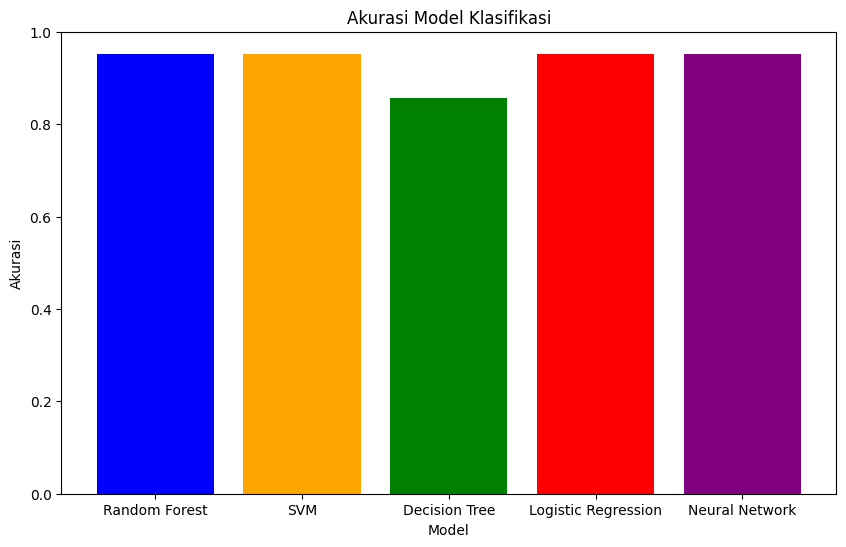
\includegraphics{Zoo0_files/figure-pdf/cell-30-output-1.png}

}

\end{figure}

Save Model

\begin{Shaded}
\begin{Highlighting}[]
\ImportTok{import}\NormalTok{ pickle}
\CommentTok{\# save model}
\ControlFlowTok{with} \BuiltInTok{open}\NormalTok{(}\StringTok{"svm\_model.pkl"}\NormalTok{, }\StringTok{"wb"}\NormalTok{) }\ImportTok{as} \BuiltInTok{file}\NormalTok{:}
\NormalTok{    pickle.dump(svm\_clf, }\BuiltInTok{file}\NormalTok{)}
\end{Highlighting}
\end{Shaded}




\backmatter
\printindex

\end{document}
